\section{Desempenho nos Datasets de Benchmark (Resultados Offline)}
\label{sec:desempenho_benchmark}

A validação empírica da arquitetura **ALF-MoE** foi conduzida sob um protocolo rigoroso de teste em partições estritamente desacopladas (\emph{offline test sets}), cobrindo os quatro conjuntos de dados analisados em sete configurações experimentais independentes. Este protocolo permitiu avaliar: (i) a capacidade de discriminação sob diferentes níveis de abstração semântica (\emph{Threat Levels} 0 e 2); (ii) a resiliência do modelo diante de falhas de rotulação em dados legados e o ganho obtido após a sanitização SOTA de \citeonline{liu2022error}; e (iii) a contribuição individual de cada especialista neural versus a representação integrada alcançada pelo bloco atencional ALF.


\subsection{Análise por Classe e Desempenho Global}
\label{subsec:analise_classe_global}

A Tabela~\ref{tab:desempenho_global_7cenarios} consolida os resultados quantitativos globais do modelo ALF-MoE em todas as matrizes experimentais avaliadas. As métricas reportadas englobam Acurácia Global ($\mathrm{Acc}$), Macro $F_1$-Score ($F_1^{\mathrm{macro}}$), Macro Precisão ($\mathrm{Prec}_{\mathrm{macro}}$), Macro Sensibilidade ($\mathrm{Rec}_{\mathrm{macro}}$), Latência por Amostra ($L_{\mathrm{sample}}$) e Vazão de Inferência ($\mathrm{Throughput}$).

\begin{table}[htb]
\centering
\caption{Desempenho global consolidado do modelo ALF-MoE nos 7 cenários de benchmark.}
\label{tab:desempenho_global_7cenarios}
\footnotesize
\setlength{\tabcolsep}{3.5pt}
\begin{tabularx}{\textwidth}{>{\raggedright\arraybackslash}X l rrrrrr}
\hline
\textbf{Conjunto de Dados} & \textbf{Cenário} & \textbf{Acurácia} & \textbf{Macro $F_1$} & \textbf{Precisão} & \textbf{Recall} & \textbf{Latência} & \textbf{Vazão} \\
\hline
CIC-UNSW-NB15 & L0 (10 cls) & 75,11\% & 0,5069 & 0,5103 & 0,6087 & 0,0479\,ms & 20.896\,fl/s \\
CIC-BCCC-NRC-2024 & L0 (49 cls) & 82,29\% & 0,4501 & 0,4505 & 0,5095 & 0,0184\,ms & 54.258\,fl/s \\
CIC-BCCC-NRC-2024 & L2 (9 cls) & 92,83\% & 0,8476 & 0,8382 & 0,8617 & 0,0122\,ms & 82.129\,fl/s \\
CSE-CIC-IDS2018 (Orig.) & L0 (15 cls) & 98,96\% & 0,8773 & 0,9045 & 0,8669 & 0,0119\,ms & 84.135\,fl/s \\
CSE-CIC-IDS2018 (Orig.) & L2 (7 cls) & 98,38\% & 0,9050 & 0,9658 & 0,8855 & 0,0111\,ms & 90.017\,fl/s \\
CSE-CIC-IDS2018 (Corr.) & L0 (15 cls) & 99,97\% & 0,8918 & 0,8814 & 0,9144 & 0,0162\,ms & 61.765\,fl/s \\
CSE-CIC-IDS2018 (Corr.) & L2 (9 cls) & 99,96\% & 0,8851 & 0,9579 & 0,8927 & 0,0118\,ms & 84.858\,fl/s \\
\hline
\end{tabularx}
\fonte{Elaborado pelo autor (2026), a partir dos relatórios experimentais.}
\end{table}

A análise comparativa dos resultados experimentais desdobra-se em três eixos centrais de discussão:

\subsubsection{Eixo 1: Impacto da Granularidade de Ameaças (Nível 0 vs. Nível 2)}

A transição entre o Nível de Ameaça 0 (classes brutas com assinaturas estritas) e o Nível de Ameaça 2 (meta-categorias operacionais consolidadas) evidencia o custo estatístico da discriminação em espaços de classes hiper-fragmentados:
\begin{itemize}
    \item No ambiente IoT (\textbf{CIC-BCCC-NRC-2024}), a consolidação de 49 classes granulares em 9 macro-famílias proporcionou uma elevação substantiva no Macro $F_1$-Score, saltando de $0{,}4501$ para $0{,}8476$ (um incremento relativo de $+88{,}3\%$), acompanhado pelo aumento da Acurácia Global de $82{,}29\%$ para $92{,}83\%$. No nível granular (L0), o modelo é compelido a distinguir entre 12 variantes microscópicas de varredura e múltiplas ramificações de inundações ICMP/UDP cuja separabilidade estatística no nível de fluxo agregado é tênue, muitas com suporte inferior a 200 instâncias de teste. Ao agregar essas variantes em famílias funcionais (como \emph{Reconnaissance}, \emph{DDoS} e \emph{IoT/MQTT}), a incerteza intra-classe é eliminada, gerando um modelo de altíssima confiabilidade operacional para acionamento perimetral;
    \item Em termos de eficiência computacional, a redução do espaço de saída no CIC-BCCC-NRC-2024 aliviou a carga de computação da projeção linear final, reduzindo a latência de $0{,}0184\,\mathrm{ms}$ para $0{,}0122\,\mathrm{ms}$ por fluxo e elevando a vazão sustentada de $54.258$ para $82.129\,\mathrm{fluxos/s}$.
\end{itemize}

\subsubsection{Eixo 2: Impacto da Sanitização de Rótulos de Liu et al. (2022) no CSE-CIC-IDS2018}

O contraste direto entre o CSE-CIC-IDS2018 Canônico e a versão corrigida segundo \citeonline{liu2022error} elucida de forma categórica as consequências do ruído de rotulação em modelos de aprendizado profundo:
\begin{itemize}
    \item Na versão original canônica (L0), o modelo atinge $98{,}96\%$ de acurácia global com Macro $F_1$ de $0{,}8773$. Contudo, a inspeção detalhada por classe revela anomalias críticas: a classe \emph{FTP-BruteForce} obteve $F_1$ de $0{,}7344$ e precisão de apenas $0{,}6843$. Essa degradação decorre diretamente da falha de etiquetagem comprovada por \citeonline{liu2022error}, na qual o servidor na porta 21 estava inativo e respondia com pacotes de encerramento \texttt{[RST, ACK]}. O classificador era forçado a aprender que respostas legítimas de porta fechada equivaliam a força bruta ativa, gerando confusão sistemática com o tráfego normal;
    \item Na versão corrigida (\emph{CSE-CIC-IDS2018 Improved}), na qual fluxos com portas fechadas e tentativas inócuas foram reclassificados como benignos, a Acurácia Global alcançou expressivos $99{,}97\%$ e o Weighted $F_1$-Score atingiu $0{,}9997$ no teste independente de 1.263.903 fluxos;
    \item Além disso, a desagregação da infiltração em classes específicas permitiu constatar que o modelo detecta varreduras internas (\emph{Infiltration - NMAP Portscan}) com $F_1 = 0{,}9912$ e canais de comando vítima-atacante com $F_1 = 0{,}8636$. Em contrapartida, a exfiltração pontual em tráfego criptografado (\emph{Infiltration - Dropbox Download}), representada por meras 17 amostras de teste, obteve $F_1 = 0{,}1818$, demonstrando que conexões legítimas a serviços de nuvem HTTPS constituem o vetor de maior furtividade para extratores baseados puramente em estatísticas de fluxo sem inspeção de carga útil.
\end{itemize}

\subsubsection{Eixo 3: Generalização em Tráfego de Alta Densidade (CIC-UNSW-NB15)}

No conjunto CIC-UNSW-NB15, que não sofreu agregação em níveis superiores (operando estritamente em L0 com 10 classes), o ALF-MoE alcançou Acurácia Global de $75{,}11\%$ e Macro $F_1$-Score de $0{,}5069$. Em classes de tráfego volumétrico e ataques de penetração complexos, o modelo exibiu excelente discriminação: \emph{Benign} ($F_1 = 0{,}9495$), \emph{Fuzzers} ($F_1 = 0{,}6968$), \emph{Exploits} ($F_1 = 0{,}6876$) e \emph{Reconnaissance} ($F_1 = 0{,}7169$). 

Para categorias com suporte diminuto, a função de perda Focal Loss balanceada priorizou a sensibilidade em detrimento da precisão: na classe \emph{Analysis} (suporte 77), o modelo obteve Sensibilidade (\emph{Recall}) de $0{,}9481$ (Acurácia Balanceada de $0{,}9661$), prevenindo a omissão do ataque embora gerando falsos positivos que reduziram o $F_1$ para $0{,}2479$. Esse comportamento reflete a postura conservadora deliberadamente imposta pelo fator de foco da Focal Loss, indispensável para ambientes corporativos em que o custo de um falso negativo (uma invasão ignorada) é infinitamente superior ao de uma inspeção secundária de falso positivo.

\subsubsection{Matrizes de Confusão Normalizadas}

A Figura~\ref{fig:matrizes_confusao_painel} reúne as matrizes de confusão normalizadas para os quatro conjuntos de dados representativos: (a) CSE-CIC-IDS2018 Canônico (L2); (b) CSE-CIC-IDS2018 Corrigido (L2); (c) CIC-BCCC-NRC-2024 (L2); e (d) CIC-UNSW-NB15 (L0).

\begin{figure}[htb]
\centering
\caption{Painel comparativo de matrizes de confusão normalizadas nos quatro cenários de avaliação.}
\label{fig:matrizes_confusao_painel}
\begin{subfigure}[b]{0.48\textwidth}
    \centering
    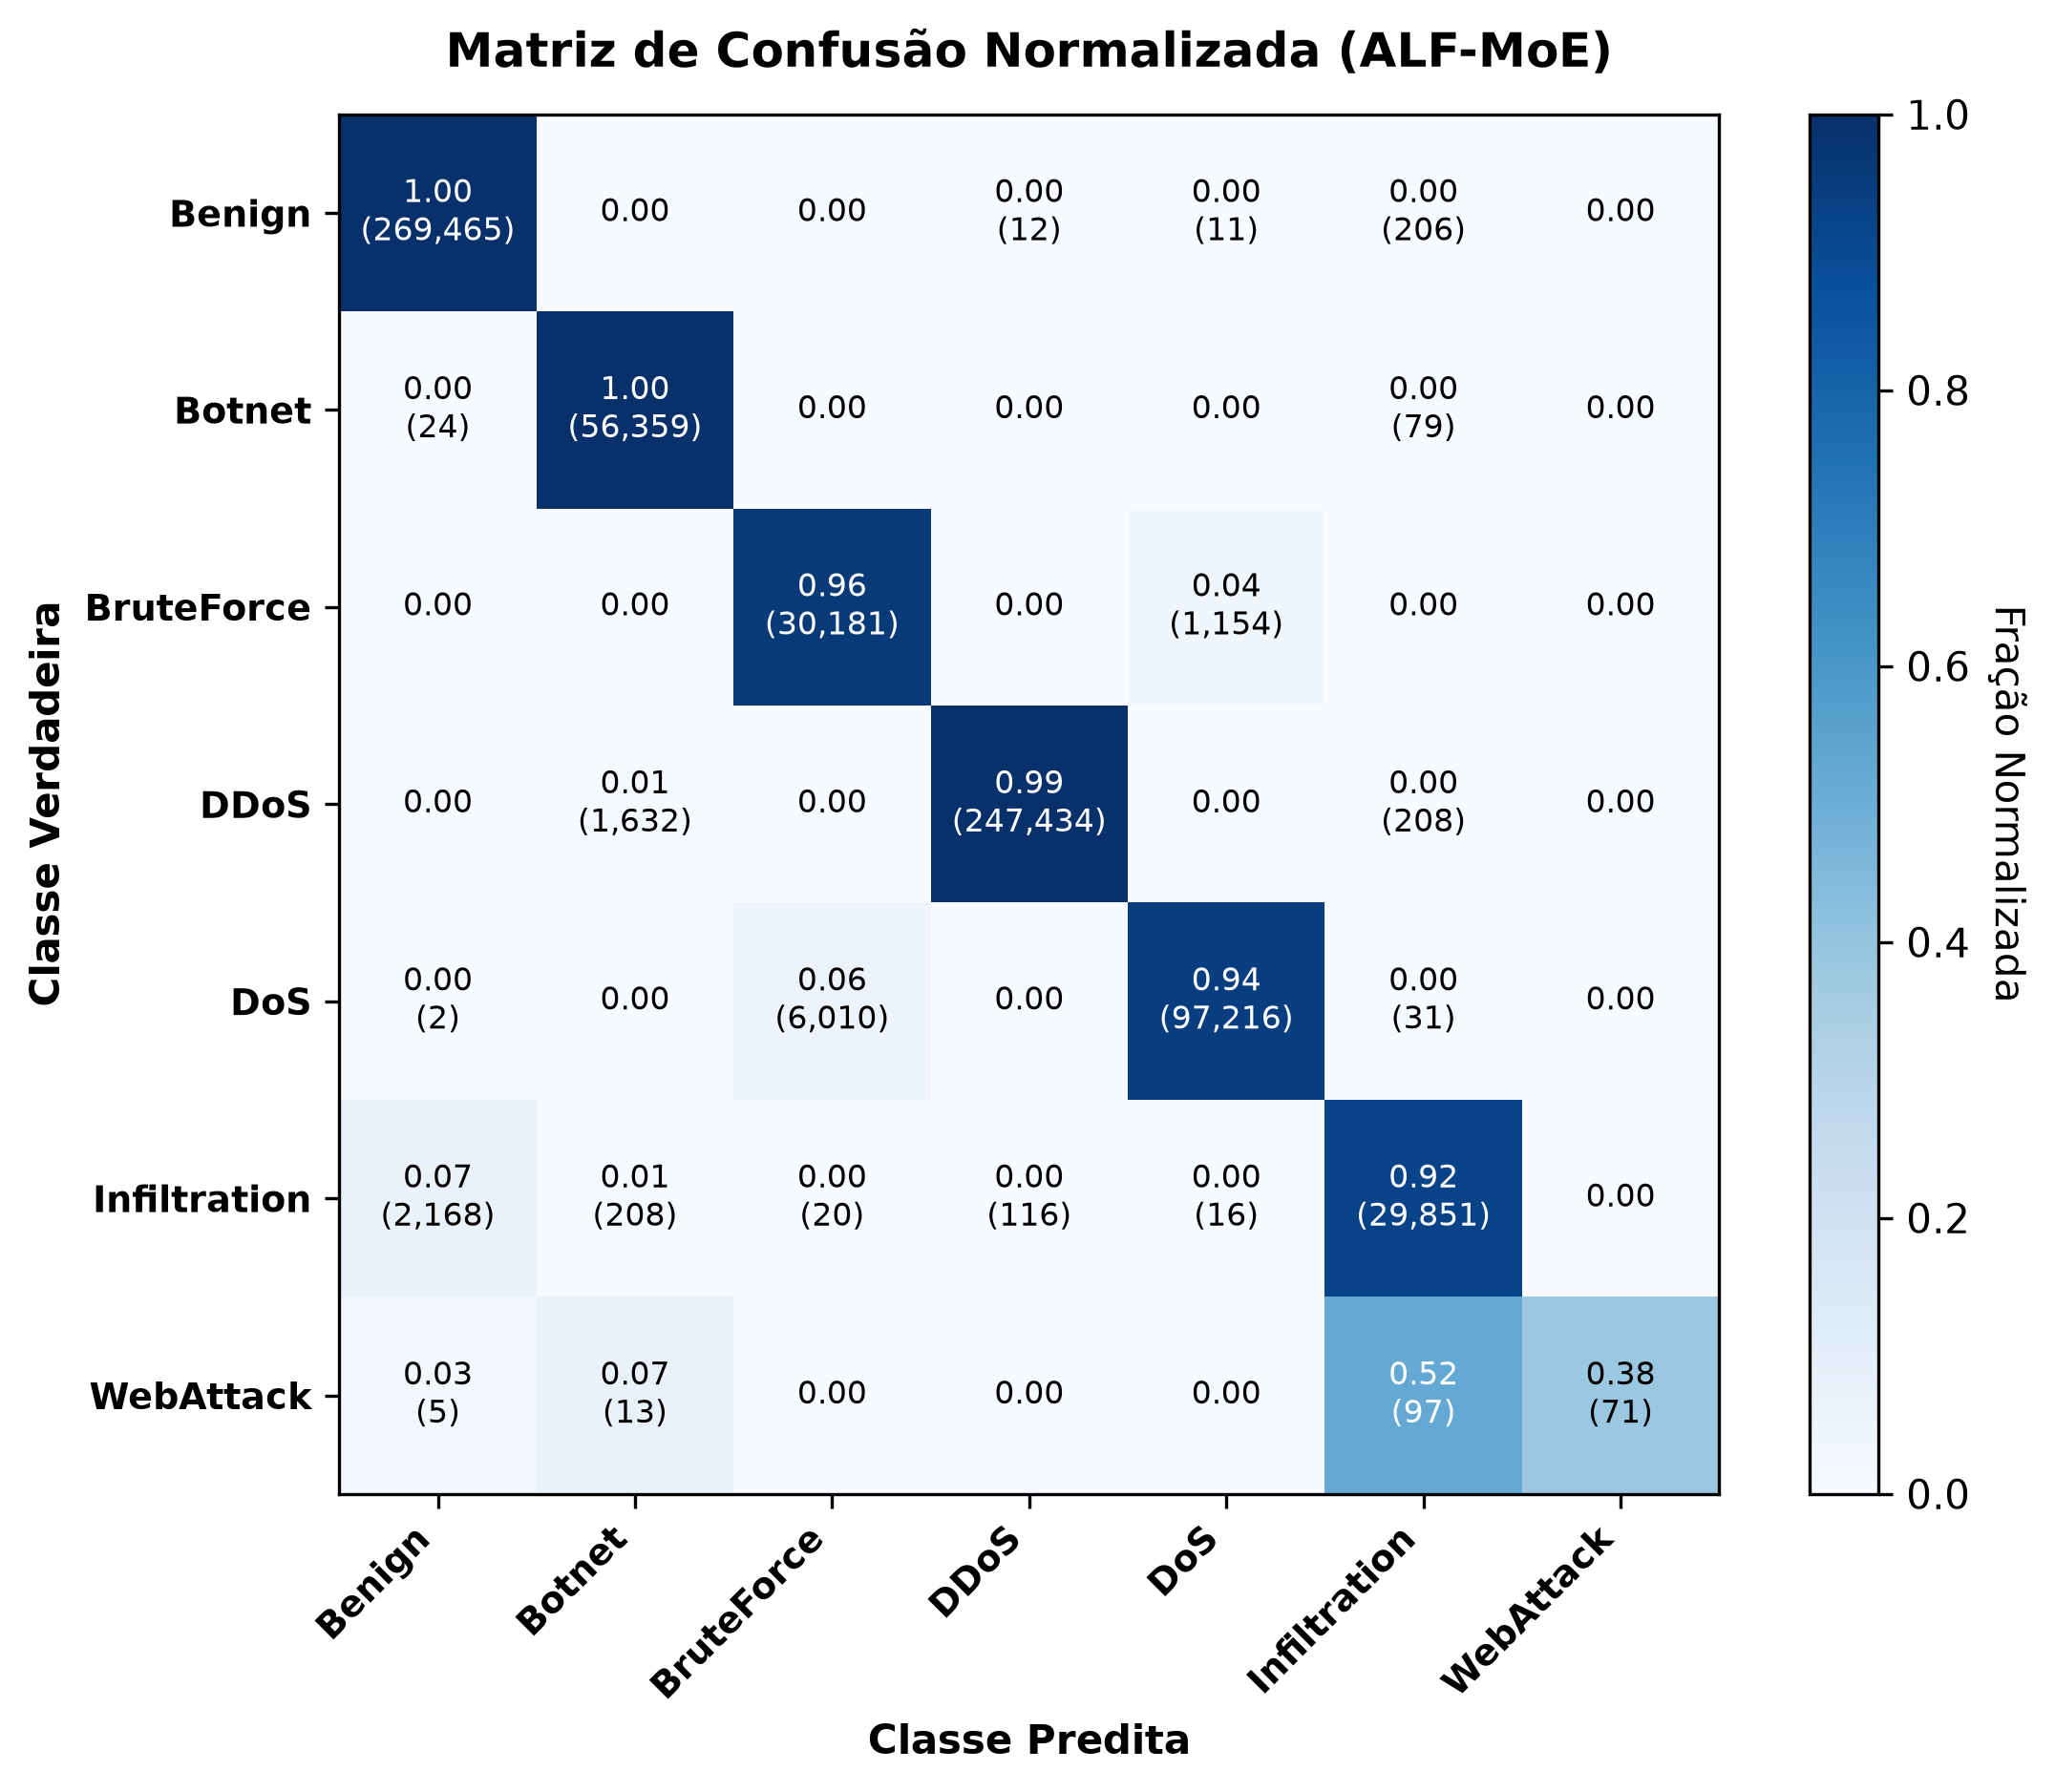
\includegraphics[width=\textwidth]{figures/benchmarks/cm_norm_cse2018_l2.png}
    \caption{CSE-CIC-IDS2018 Canônico (L2 - 7 classes).}
    \label{subfig:cm_cse2018_orig}
\end{subfigure}
\hfill
\begin{subfigure}[b]{0.48\textwidth}
    \centering
    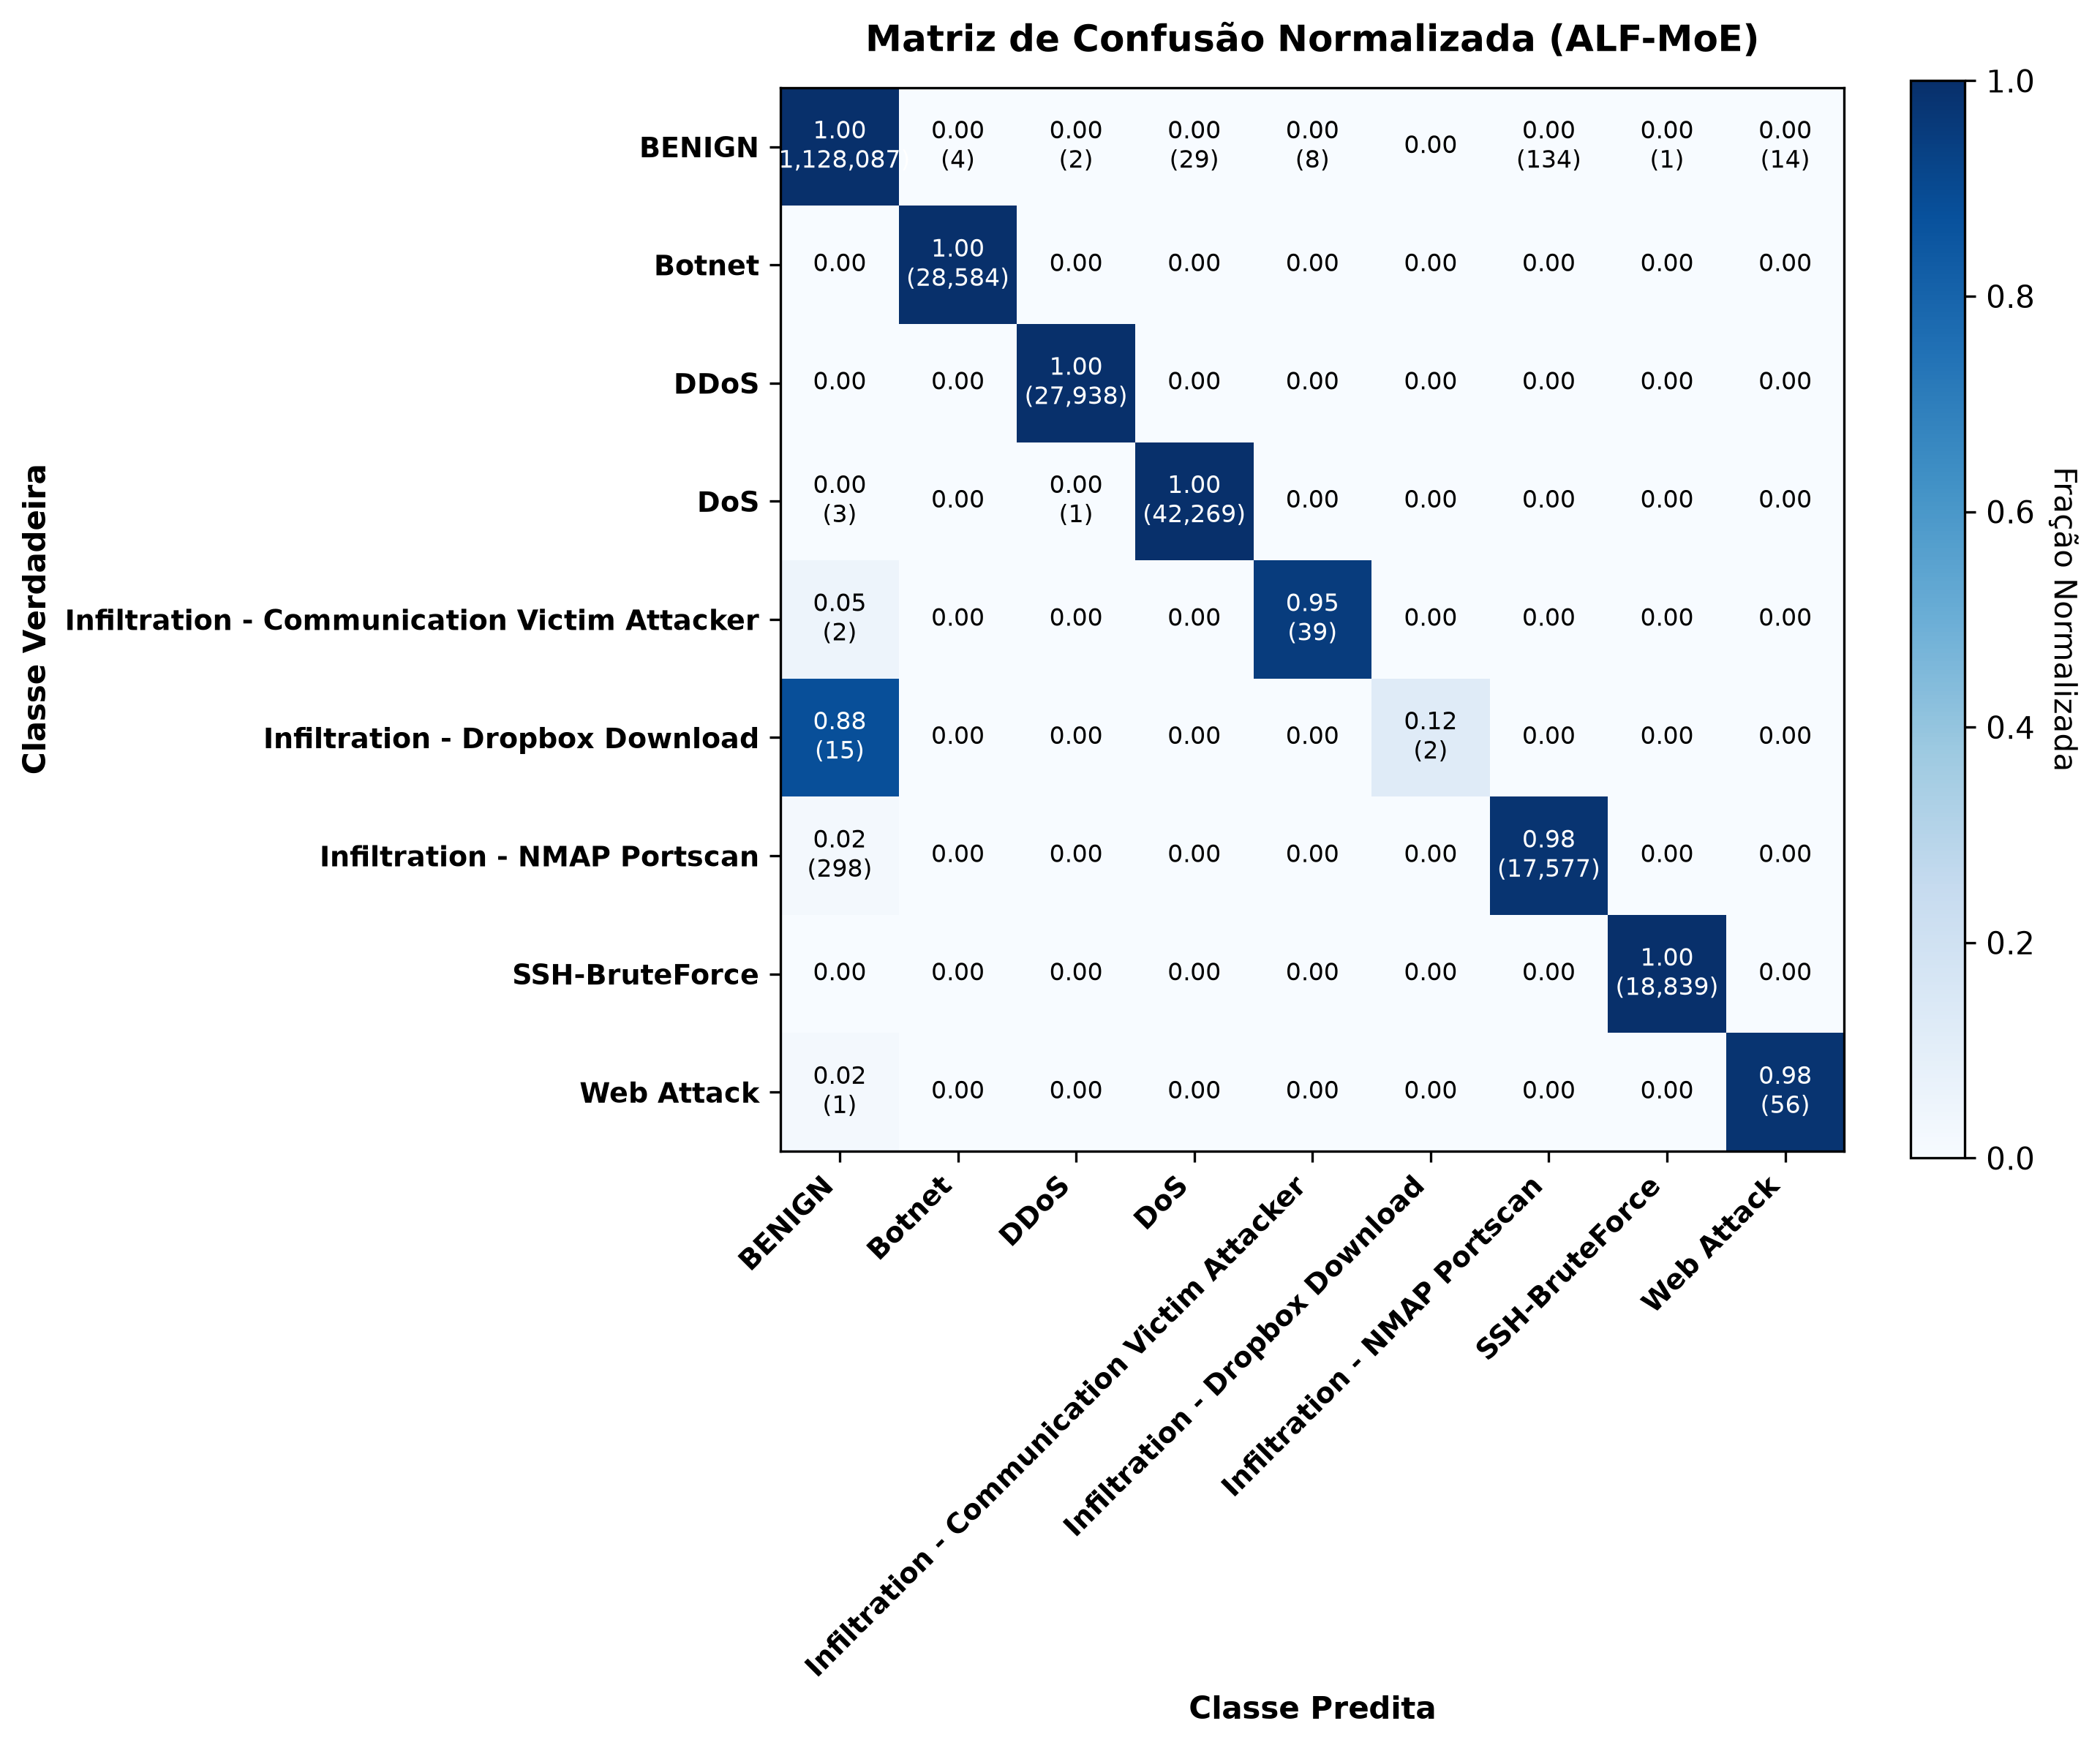
\includegraphics[width=\textwidth]{figures/benchmarks/cm_norm_cse2018_imp_l2.png}
    \caption{CSE-CIC-IDS2018 Corrigido (L2 - 9 classes).}
    \label{subfig:cm_cse2018_imp}
\end{subfigure}

\vspace{0.4cm}

\begin{subfigure}[b]{0.48\textwidth}
    \centering
    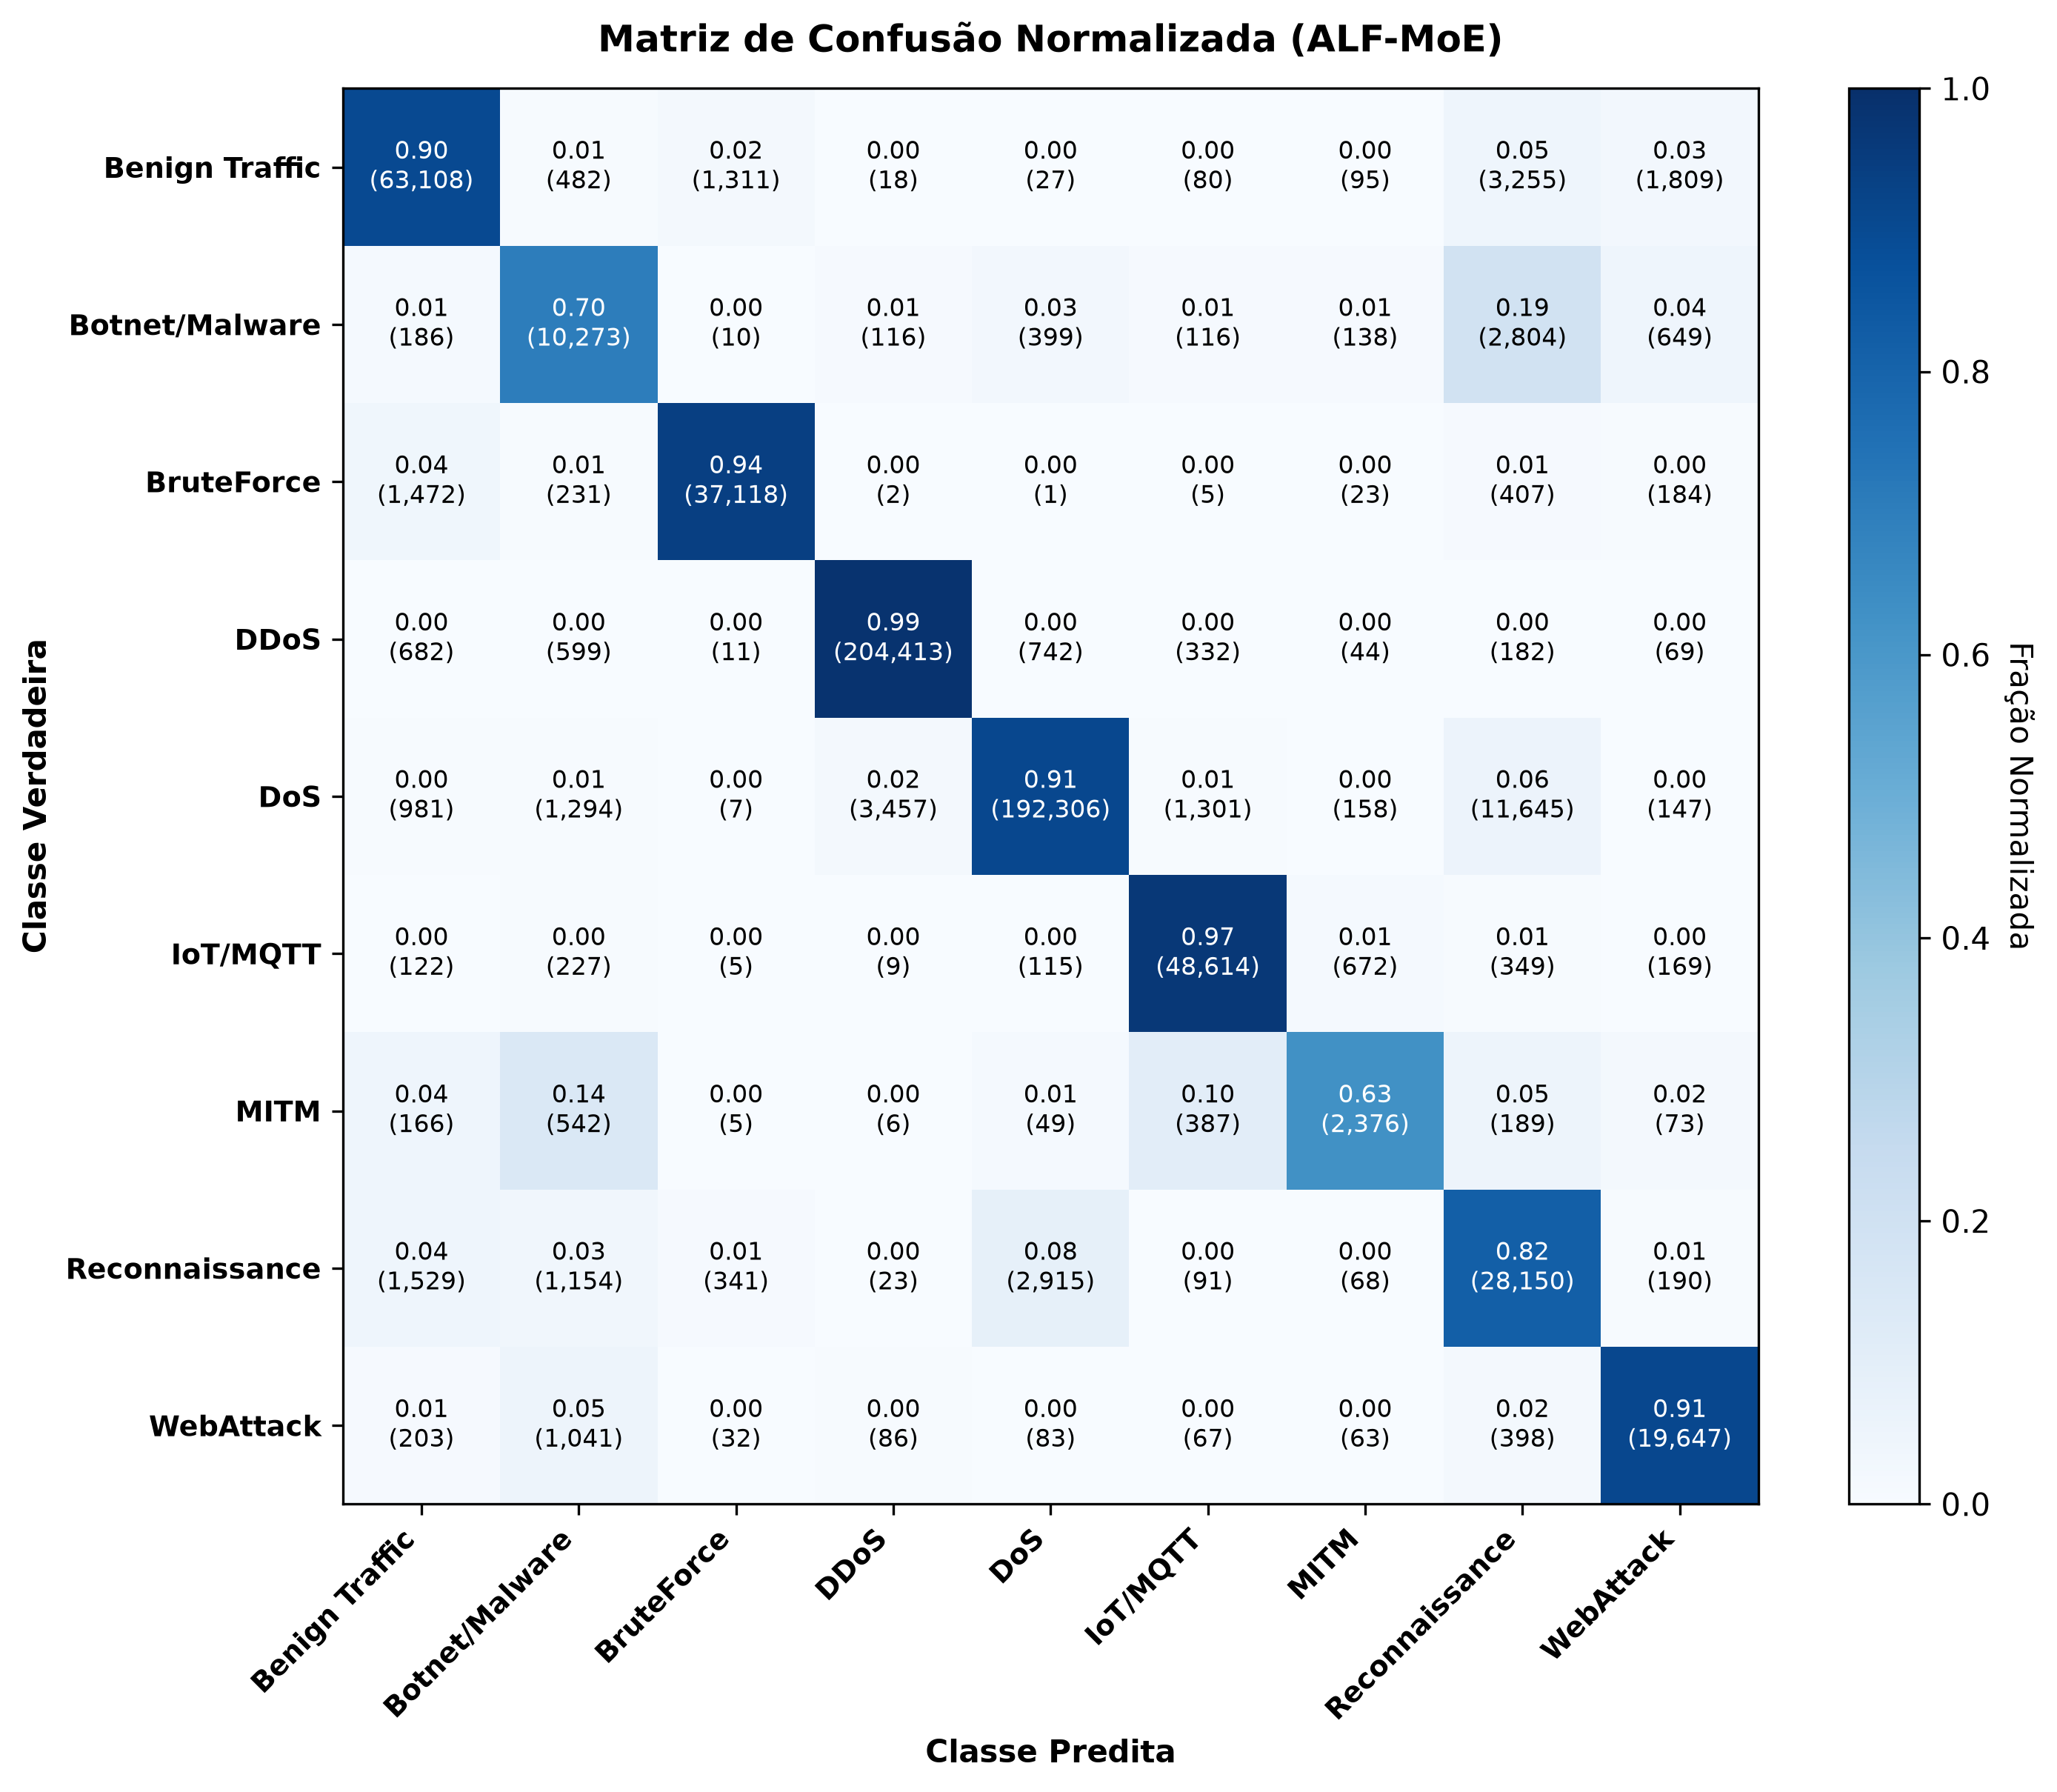
\includegraphics[width=\textwidth]{figures/benchmarks/cm_norm_bccc2024_l2.png}
    \caption{CIC-BCCC-NRC-2024 (L2 - 9 classes).}
    \label{subfig:cm_bccc2024}
\end{subfigure}
\hfill
\begin{subfigure}[b]{0.48\textwidth}
    \centering
    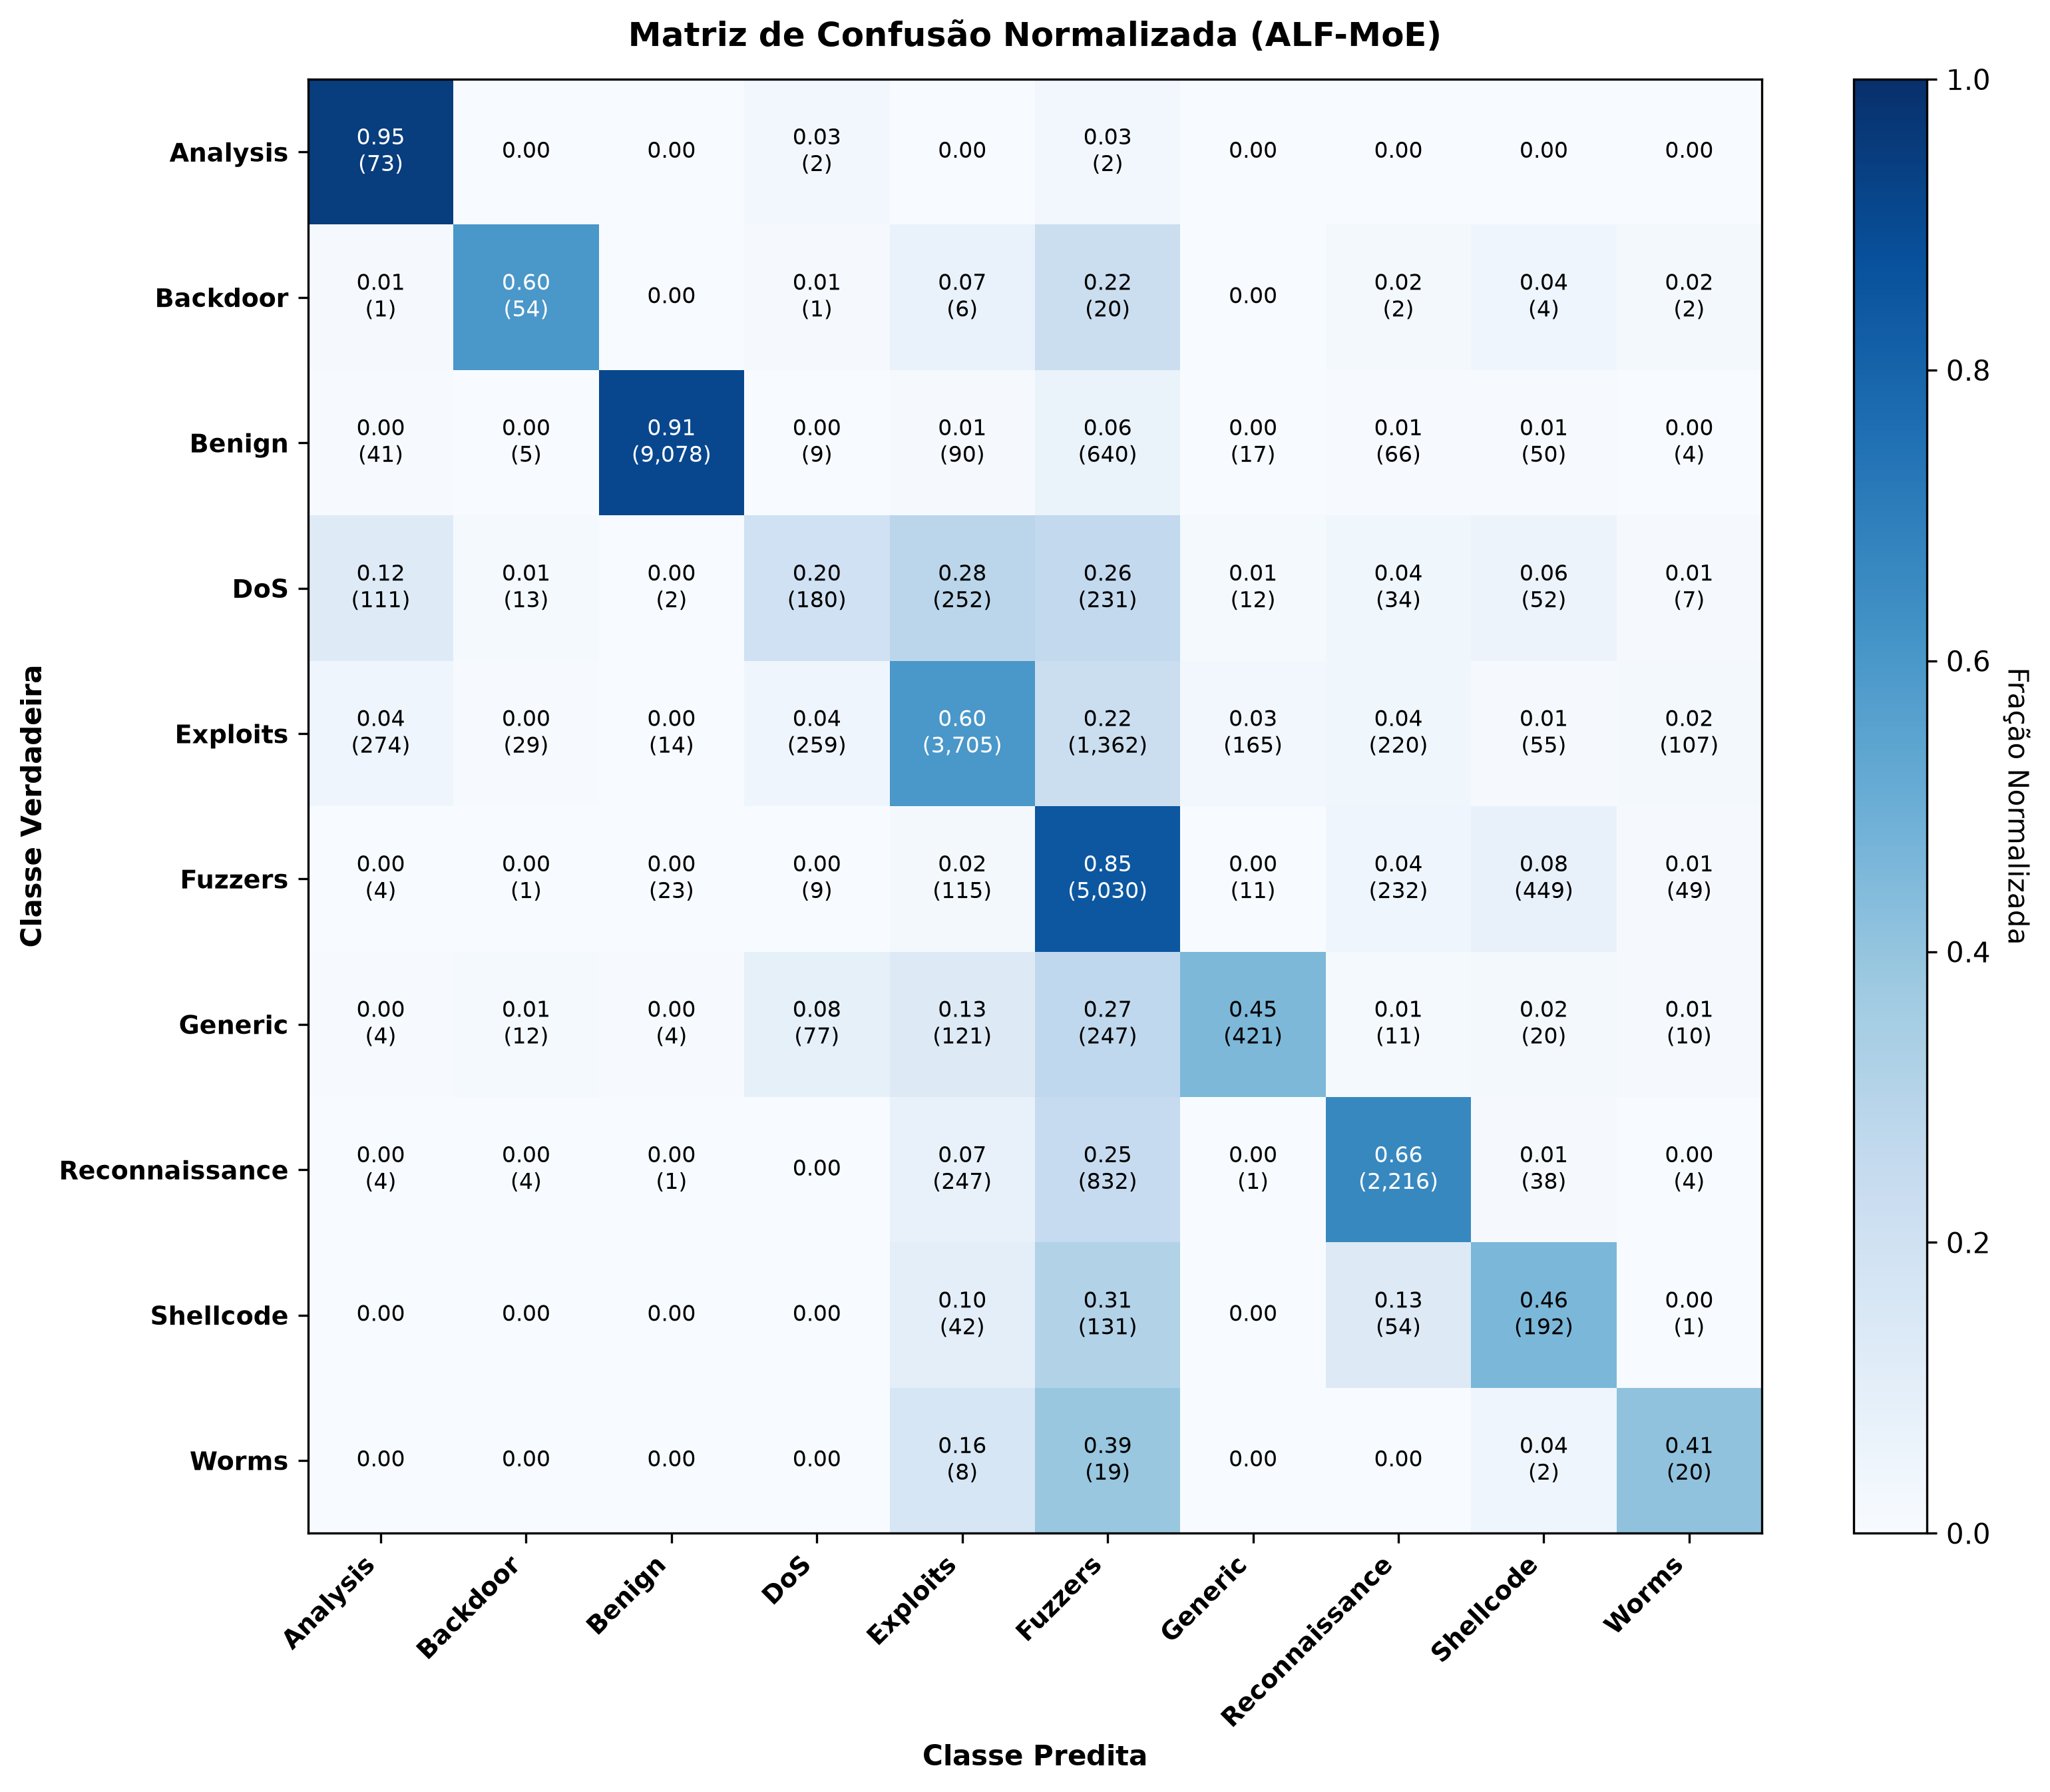
\includegraphics[width=\textwidth]{figures/benchmarks/cm_norm_unsw_l0.png}
    \caption{CIC-UNSW-NB15 (L0 - 10 classes).}
    \label{subfig:cm_unsw}
\end{subfigure}
\fonte{Elaborado pelo autor (2026), a partir dos artefatos de avaliação.}
\end{figure}

A inspeção visual confirma a dominância quase diagonal absoluta na versão corrigida do CSE-CIC-IDS2018 (Figura~\ref{subfig:cm_cse2018_imp}), em contraste com a dispersão de erros verificada na versão original (Figura~\ref{subfig:cm_cse2018_orig}). No ambiente IoT (Figura~\ref{subfig:cm_bccc2024}), observa-se perfeita segregação de tráfego de intermediadores MQTT ($96{,}0\%$ de acerto) e inundações DoS/DDoS ($>94\%$), enquanto o UNSW-NB15 (Figura~\ref{subfig:cm_unsw}) ilustra a sobreposição natural existente entre as classes \emph{Exploits} e \emph{Fuzzers}.

A análise pormenorizada das dispersões fora da diagonal principal permite fundamentar quatro padrões específicos de confusão interclasses observados nos experimentos, balizados pelas restrições físico-matemáticas da telemetria de fluxo:
\begin{enumerate}
    \item \textbf{CSE-CIC-IDS2018 Canônico (\emph{Infiltration} vs. \emph{WebAttack}):}
    Verifica-se sobreposição estatística mútua entre fluxos de infiltração e ataques a aplicações web. Essa confusão decorre do fato de ambos os vetores operarem predominantemente sobre os protocolos de transporte das portas 80 (HTTP) e 443 (HTTPS), compartilhando assinaturas idênticas de cabeçalho TCP e cadência de requisições. Como os extratores NetFlow/CICFlowMeter descartam o conteúdo da carga útil (\emph{payload}), a diferenciação apoia-se unicamente em distribuições de tamanho e temporização de pacotes. Além disso, a classe \emph{WebAttack} no conjunto canônico conta com suporte diminuto de teste (apenas 186 instâncias somando \emph{Brute Force - Web}, \emph{Brute Force - XSS} e \emph{SQL Injection}), limitando a estimativa das fronteiras bayesianas de decisão;
    
    \item \textbf{CSE-CIC-IDS2018 Corrigido (\emph{Benign} vs. \emph{Infiltration - Dropbox Download}):}
    Na base saneada conforme \citeonline{liu2022error}, a classe \emph{Infiltration - Dropbox Download} alcança $F_1 = 0{,}1818$ com dispersão preponderante em direção à classe \emph{Benign}. Essa confusão é tecnicamente inevitável no nível de fluxo: a exfiltração de dados e download de artefatos maliciosos via API oficial do Dropbox utiliza canais TLS legítimos em conexões HTTPS padronizadas, reproduzindo rigorosamente as grandezas estatísticas e temporais da navegação web corporativa. Aliado ao suporte ultra-reduzido de apenas 17 amostras de teste, esse vetor atinge o limite intrínseco de separabilidade de extratores estritamente baseados em fluxo de rede;
    
    \item \textbf{CIC-BCCC-NRC TabularIoTAttack-2024 (\emph{MITM} vs. \emph{Botnet}):}
    No ecossistema IoT, constata-se confusão pontual entre fluxos das macro-famílias \emph{MITM} (especialmente variantes de \emph{ARP Spoofing}) e tráfego de \emph{Botnet}. Em redes locais de sensores e atuadores, ambos os vetores caracterizam-se por mensagens curtas de controle TCP/IP, ausência de fluxos volumétricos em rajada (\emph{bulk}) e temporizações assíncronas com intervalos de inter-chegada assemelhados, induzindo dispersão correlacionada nos logits da Gating Network;
    
    \item \textbf{CIC-UNSW-NB15 (\emph{Analysis}, \emph{Backdoor}, \emph{Exploits} e \emph{Fuzzers}):}
    No benchmark UNSW-NB15, verifica-se sobreposição estatística mútua entre as classes \emph{Exploits} ($22{,}17\%$ do teste) e \emph{Fuzzers} ($21{,}22\%$), além de falsos positivos cruzados com \emph{Analysis} e \emph{Backdoor}. Conforme documentado por \citeonline{moustafa2015unsw}, o tráfego sintético dessa base foi sintetizado pelo gerador de hardware comercial IXIA PerfectStorm injetando transações HTTP padronizadas com payloads mutacionados. No plano da telemetria de fluxo (contadores agregados de pacotes, bytes e intervalos IAT), essas classes produzem vetores numéricos virtualmente idênticos, delimitando um teto teórico de erro de Bayes intransponível sem inspeção profunda de pacotes (DPI).
\end{enumerate}


\subsection{Análise Comparativa dos Especialistas e do Bloco ALF}
\label{subsec:estudo_ablacao}

A arquitetura ALF-MoE apoia-se no princípio de que especialistas neurais heterogêneos, concebidos para extrair representações de domínios específicos da telemetria de rede, oferecem projeções complementares que, ao serem integradas pela fusão por atenção adaptativa, superam a capacidade preditiva de qualquer modelo monolítico individual. Para quantificar essa premissa de projeto e mensurar o ganho advindo do bloco atencional ALF sobre os ramos isolados, realizou-se uma análise comparativa sistemática entre as predições supervisionadas das cinco cabeças especializadas ($\mathcal{E}_{\mathrm{DNN}}, \mathcal{E}_{\mathrm{CNN}}, \mathcal{E}_{\mathrm{GRU}}, \mathcal{E}_{\mathrm{CAE}}, \mathcal{E}_{\mathrm{LSTM}}$) e a predição da cabeça integrada ALF-MoE.

A Tabela~\ref{tab:estudo_ablacao_completo} sumariza o Macro $F_1$-Score e a Acurácia Global obtidos por cada especialista e pela cabeça unificada ALF nos sete cenários de teste.

\begin{table}[htb]
\centering
\caption{Estudo de ablação: Macro $F_1$-Score e Acurácia dos especialistas individuais vs. ALF-MoE.}
\label{tab:estudo_ablacao_completo}
\footnotesize
\setlength{\tabcolsep}{4.5pt}
\begin{tabularx}{\textwidth}{>{\raggedright\arraybackslash}X l rrrrrr}
\hline
\textbf{Dataset} & \textbf{Métrica} & \textbf{DNN} & \textbf{CNN} & \textbf{GRU} & \textbf{CAE} & \textbf{LSTM} & \textbf{ALF-MoE} \\
\hline
\multirow{2}{*}{CIC-UNSW-NB15 (L0)} 
 & Macro $F_1$ & 0,4611 & 0,4053 & 0,4367 & 0,2525 & 0,2779 & \textbf{0,5069} \\
 & Acurácia    & 71,77\% & 58,56\% & 71,42\% & 62,28\% & 64,12\% & \textbf{75,11\%} \\
\hline
\multirow{2}{*}{CIC-BCCC-NRC-2024 (L0)} 
 & Macro $F_1$ & 0,0057 & 0,2496 & 0,4448 & 0,1246 & 0,3676 & \textbf{0,4501} \\
 & Acurácia    & 10,88\% & 41,31\% & \textbf{82,33\%} & 60,73\% & 80,06\% & 82,29\% \\
\hline
\multirow{2}{*}{CIC-BCCC-NRC-2024 (L2)} 
 & Macro $F_1$ & 0,1284 & 0,5551 & 0,8451 & 0,2557 & 0,8163 & \textbf{0,8476} \\
 & Acurácia    & 12,41\% & 57,04\% & 92,26\% & 60,55\% & 90,88\% & \textbf{92,83\%} \\
\hline
\multirow{2}{*}{CSE-CIC-IDS2018 Orig. (L0)} 
 & Macro $F_1$ & 0,7588 & 0,5485 & 0,7681 & 0,4750 & 0,6891 & \textbf{0,8773} \\
 & Acurácia    & 93,05\% & 51,73\% & 88,62\% & 69,61\% & 89,09\% & \textbf{98,96\%} \\
\hline
\multirow{2}{*}{CSE-CIC-IDS2018 Orig. (L2)} 
 & Macro $F_1$ & 0,8442 & 0,5925 & 0,8181 & 0,3029 & 0,7880 & \textbf{0,9050} \\
 & Acurácia    & 94,30\% & 61,53\% & 88,62\% & 44,05\% & 88,13\% & \textbf{98,38\%} \\
\hline
\multirow{2}{*}{CSE-CIC-IDS2018 Corr. (L0)} 
 & Macro $F_1$ & 0,7862 & 0,7156 & 0,8390 & 0,4405 & 0,7598 & \textbf{0,8918} \\
 & Acurácia    & 99,85\% & 92,87\% & 99,40\% & 78,51\% & 98,37\% & \textbf{99,97\%} \\
\hline
\multirow{2}{*}{CSE-CIC-IDS2018 Corr. (L2)} 
 & Macro $F_1$ & 0,8134 & 0,6953 & 0,8464 & 0,5115 & 0,7344 & \textbf{0,8851} \\
 & Acurácia    & 99,85\% & 92,84\% & 99,34\% & 77,40\% & 97,77\% & \textbf{99,96\%} \\
\hline
\end{tabularx}
\fonte{Elaborado pelo autor (2026), com base nos relatórios de teste.}
\end{table}

A análise minuciosa da Tabela~\ref{tab:estudo_ablacao_completo} permite derivar conclusões estruturais acerca do comportamento dos especialistas e do ganho proporcionado pela fusão ALF:
\begin{enumerate}
    \item \textbf{Superação Sistemática do Melhor Especialista Individual:}
    Em todos os cenários sem exceção, a fusão atencional \textbf{ALF-MoE} alcança o melhor Macro $F_1$-Score global. No CIC-UNSW-NB15, o melhor especialista isolado foi a $\mathcal{E}_{\mathrm{DNN}}$ ($F_1 = 0{,}4611$), enquanto o ALF-MoE atingiu $0{,}5069$ (ganho de $+4{,}58$ pontos percentuais de $F_1$ e $+3{,}34\%$ em acurácia). No CSE-CIC-IDS2018 Canônico (L0), o ganho é ainda mais acentuado: o melhor especialista individual foi a $\mathcal{E}_{\mathrm{GRU}}$ com $F_1 = 0{,}7681$, superada largamente pelo ALF-MoE com $0{,}8773$ (um salto de $+10{,}92$ pontos de $F_1$ e $+5{,}91\%$ de acurácia sobre a DNN);
    
    \item \textbf{Especialização Funcional por Domínio:}
    Os especialistas $\mathcal{E}_{\mathrm{GRU}}$ e $\mathcal{E}_{\mathrm{LSTM}}$, encarregados da telemetria de intervalos temporais (\emph{IAT} e \emph{Active/Idle}), demonstraram liderança folgada no tráfego IoT (CIC-BCCC-NRC-2024), alcançando $F_1$ de $0{,}8451$ e $0{,}8163$, respectivamente, enquanto os modelos alimentados unicamente por propriedades de pacotes ou globais sofreram degradação. Isso decorre da natureza do protocolo MQTT, cujos pacotes apresentam tamanho uniforme de cabeçalho, tornando os padrões de tempo entre chegadas o elemento primordial de discriminação;
    
    \item \textbf{Papel Regularizador do Autoencoder Convolucional ($\mathcal{E}_{\mathrm{CAE}}$):}
    Embora o $\mathcal{E}_{\mathrm{CAE}}$ isole pontuações mais modestas como classificador autônomo (variando entre $F_1 = 0{,}1246$ e $0{,}5115$), sua inclusão no grafo computacional provê uma restrição de reconstrução espectral no domínio da frequência ($\mathcal{L}_{\mathrm{CAE\_rec}}$) que atua como regularizador indutivo, impedindo que os especialistas densos entrem em colapso latente diante de fluxos volumétricos colineares.
\end{enumerate}

\subsubsection{Gráficos Radar de Especialistas}

A complementaridade multidomínio dos modelos é visualizada na Figura~\ref{fig:radar_especialistas_painel}, que reúne os gráficos radar de comparação entre cada especialista e a arquitetura ALF-MoE nos quatro conjuntos de teste.

\begin{figure}[htb]
\centering
\caption{Gráficos radar comparativos de desempenho por classe: Especialistas individuais vs. ALF-MoE.}
\label{fig:radar_especialistas_painel}
\begin{subfigure}[b]{0.48\textwidth}
    \centering
    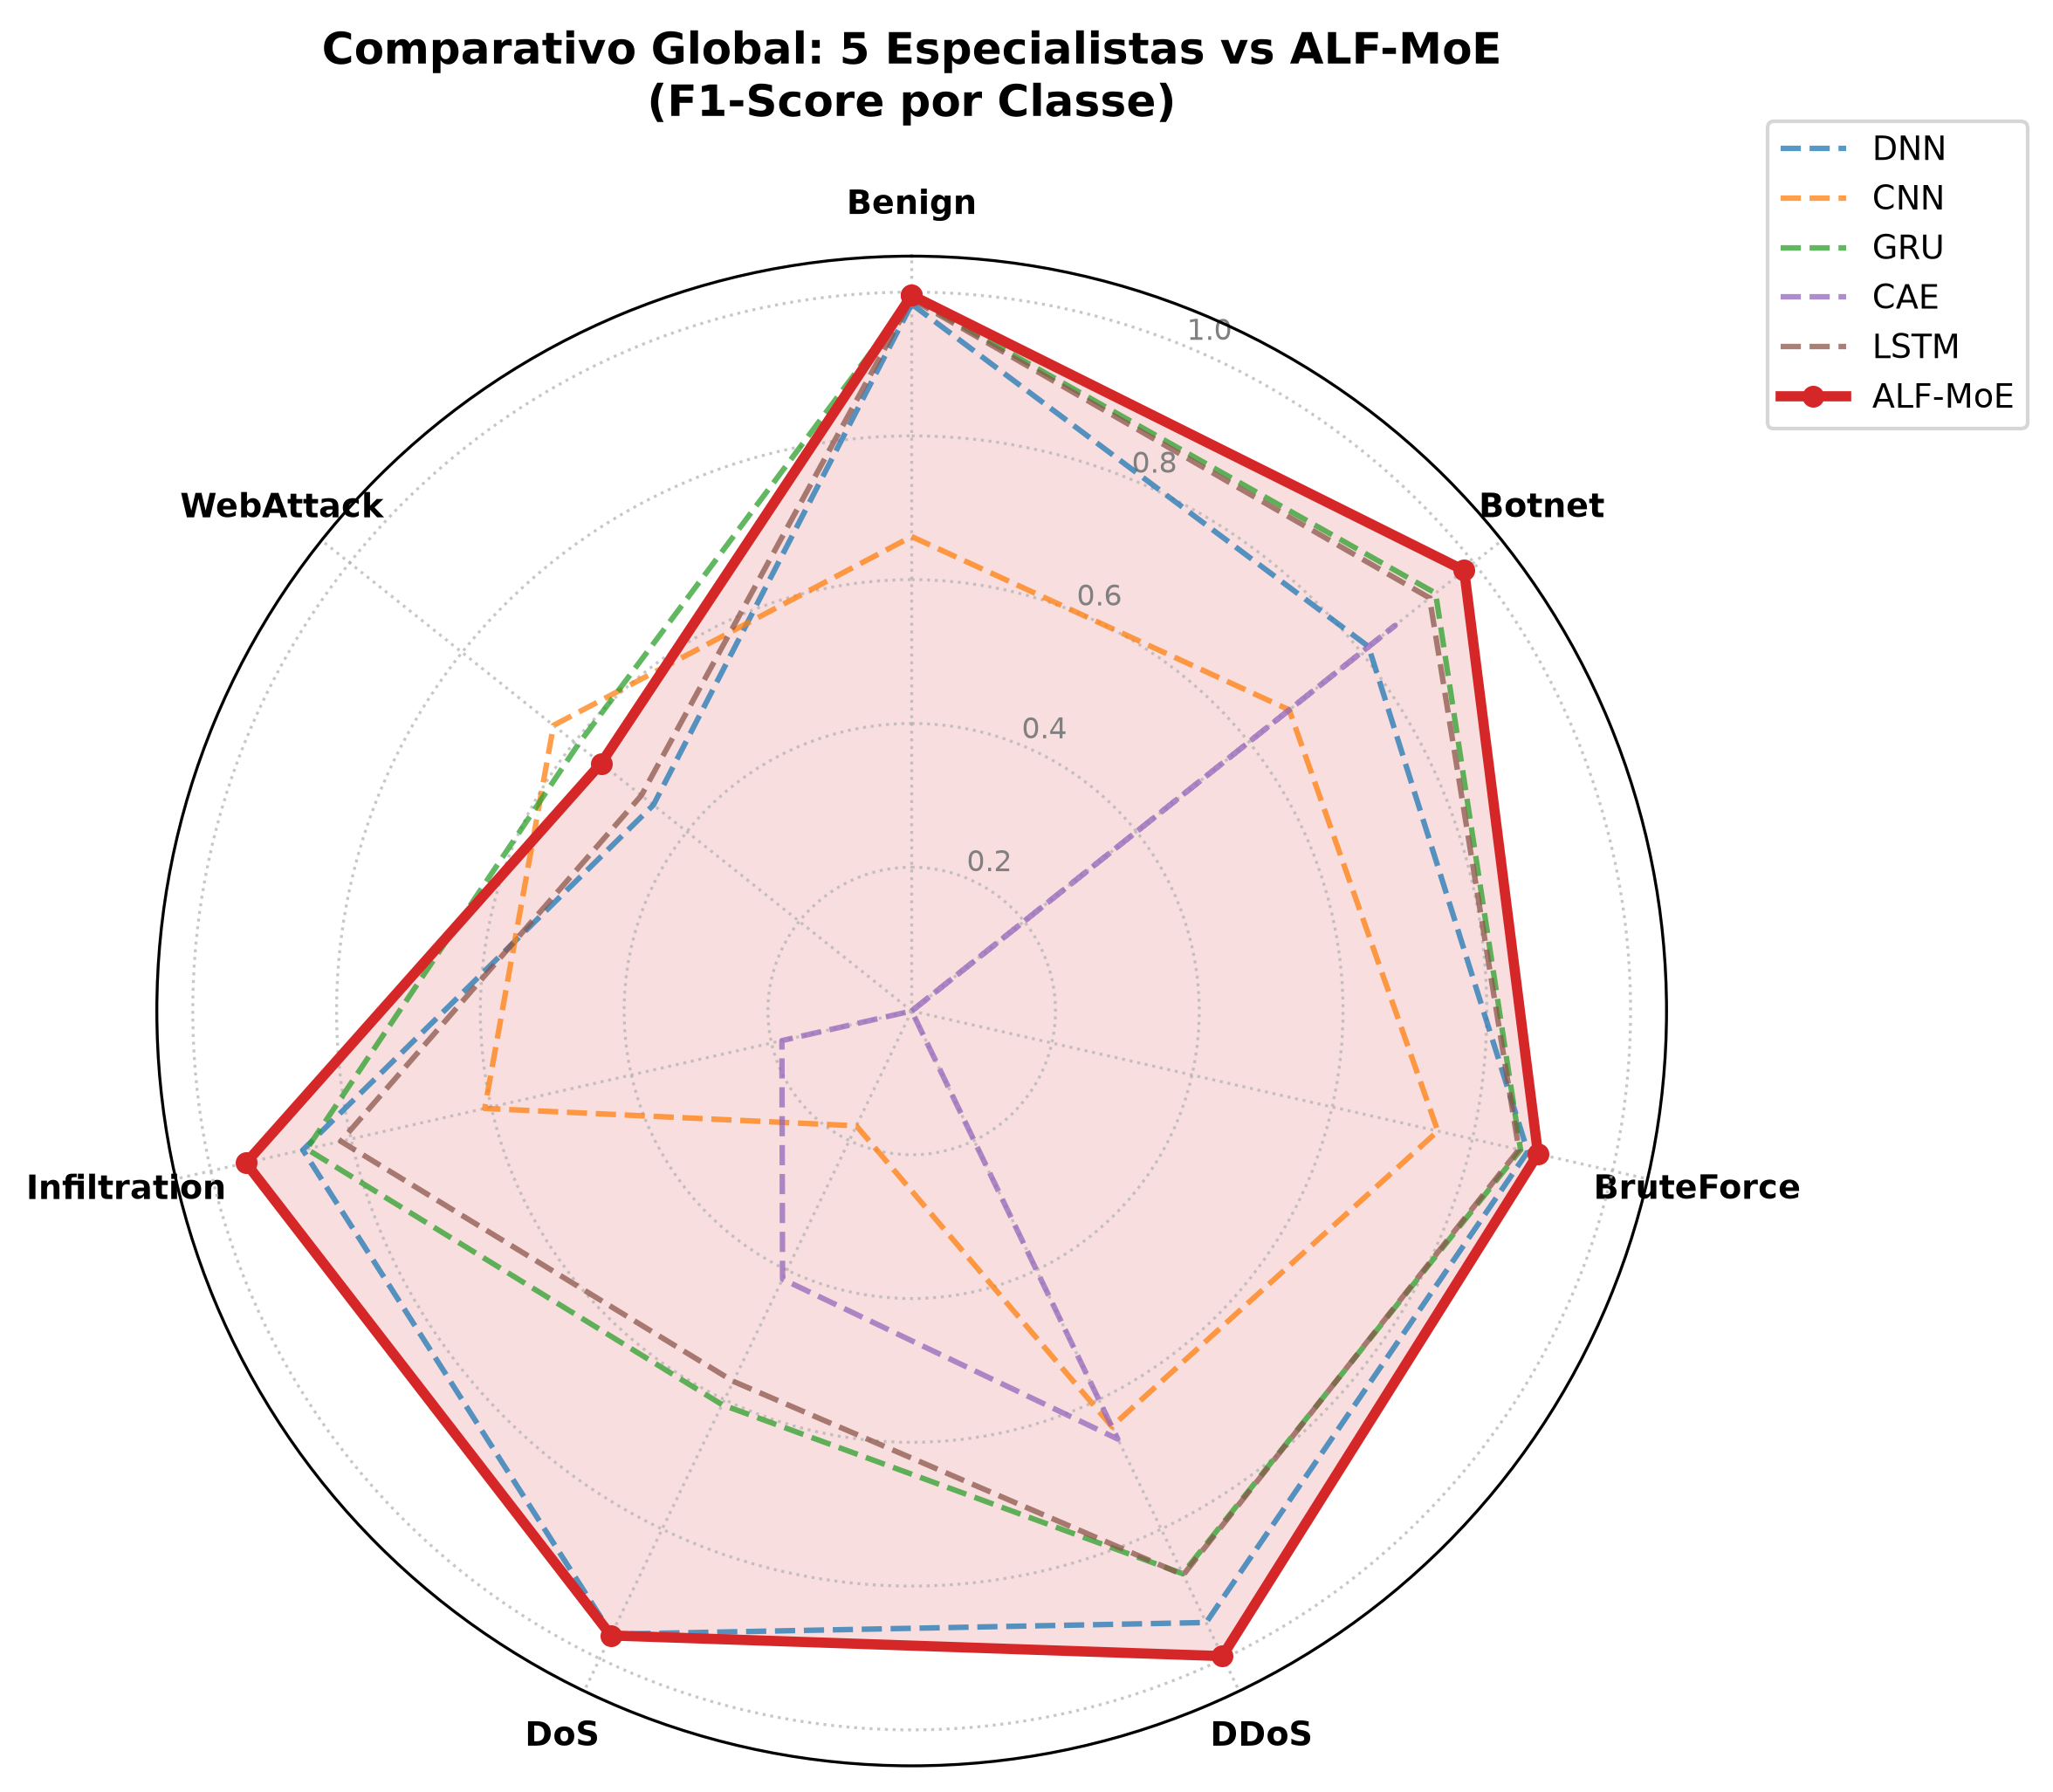
\includegraphics[width=\textwidth]{figures/benchmarks/radar_cse2018_l2.png}
    \caption{CSE-CIC-IDS2018 Canônico (L2).}
    \label{subfig:radar_cse_orig}
\end{subfigure}
\hfill
\begin{subfigure}[b]{0.48\textwidth}
    \centering
    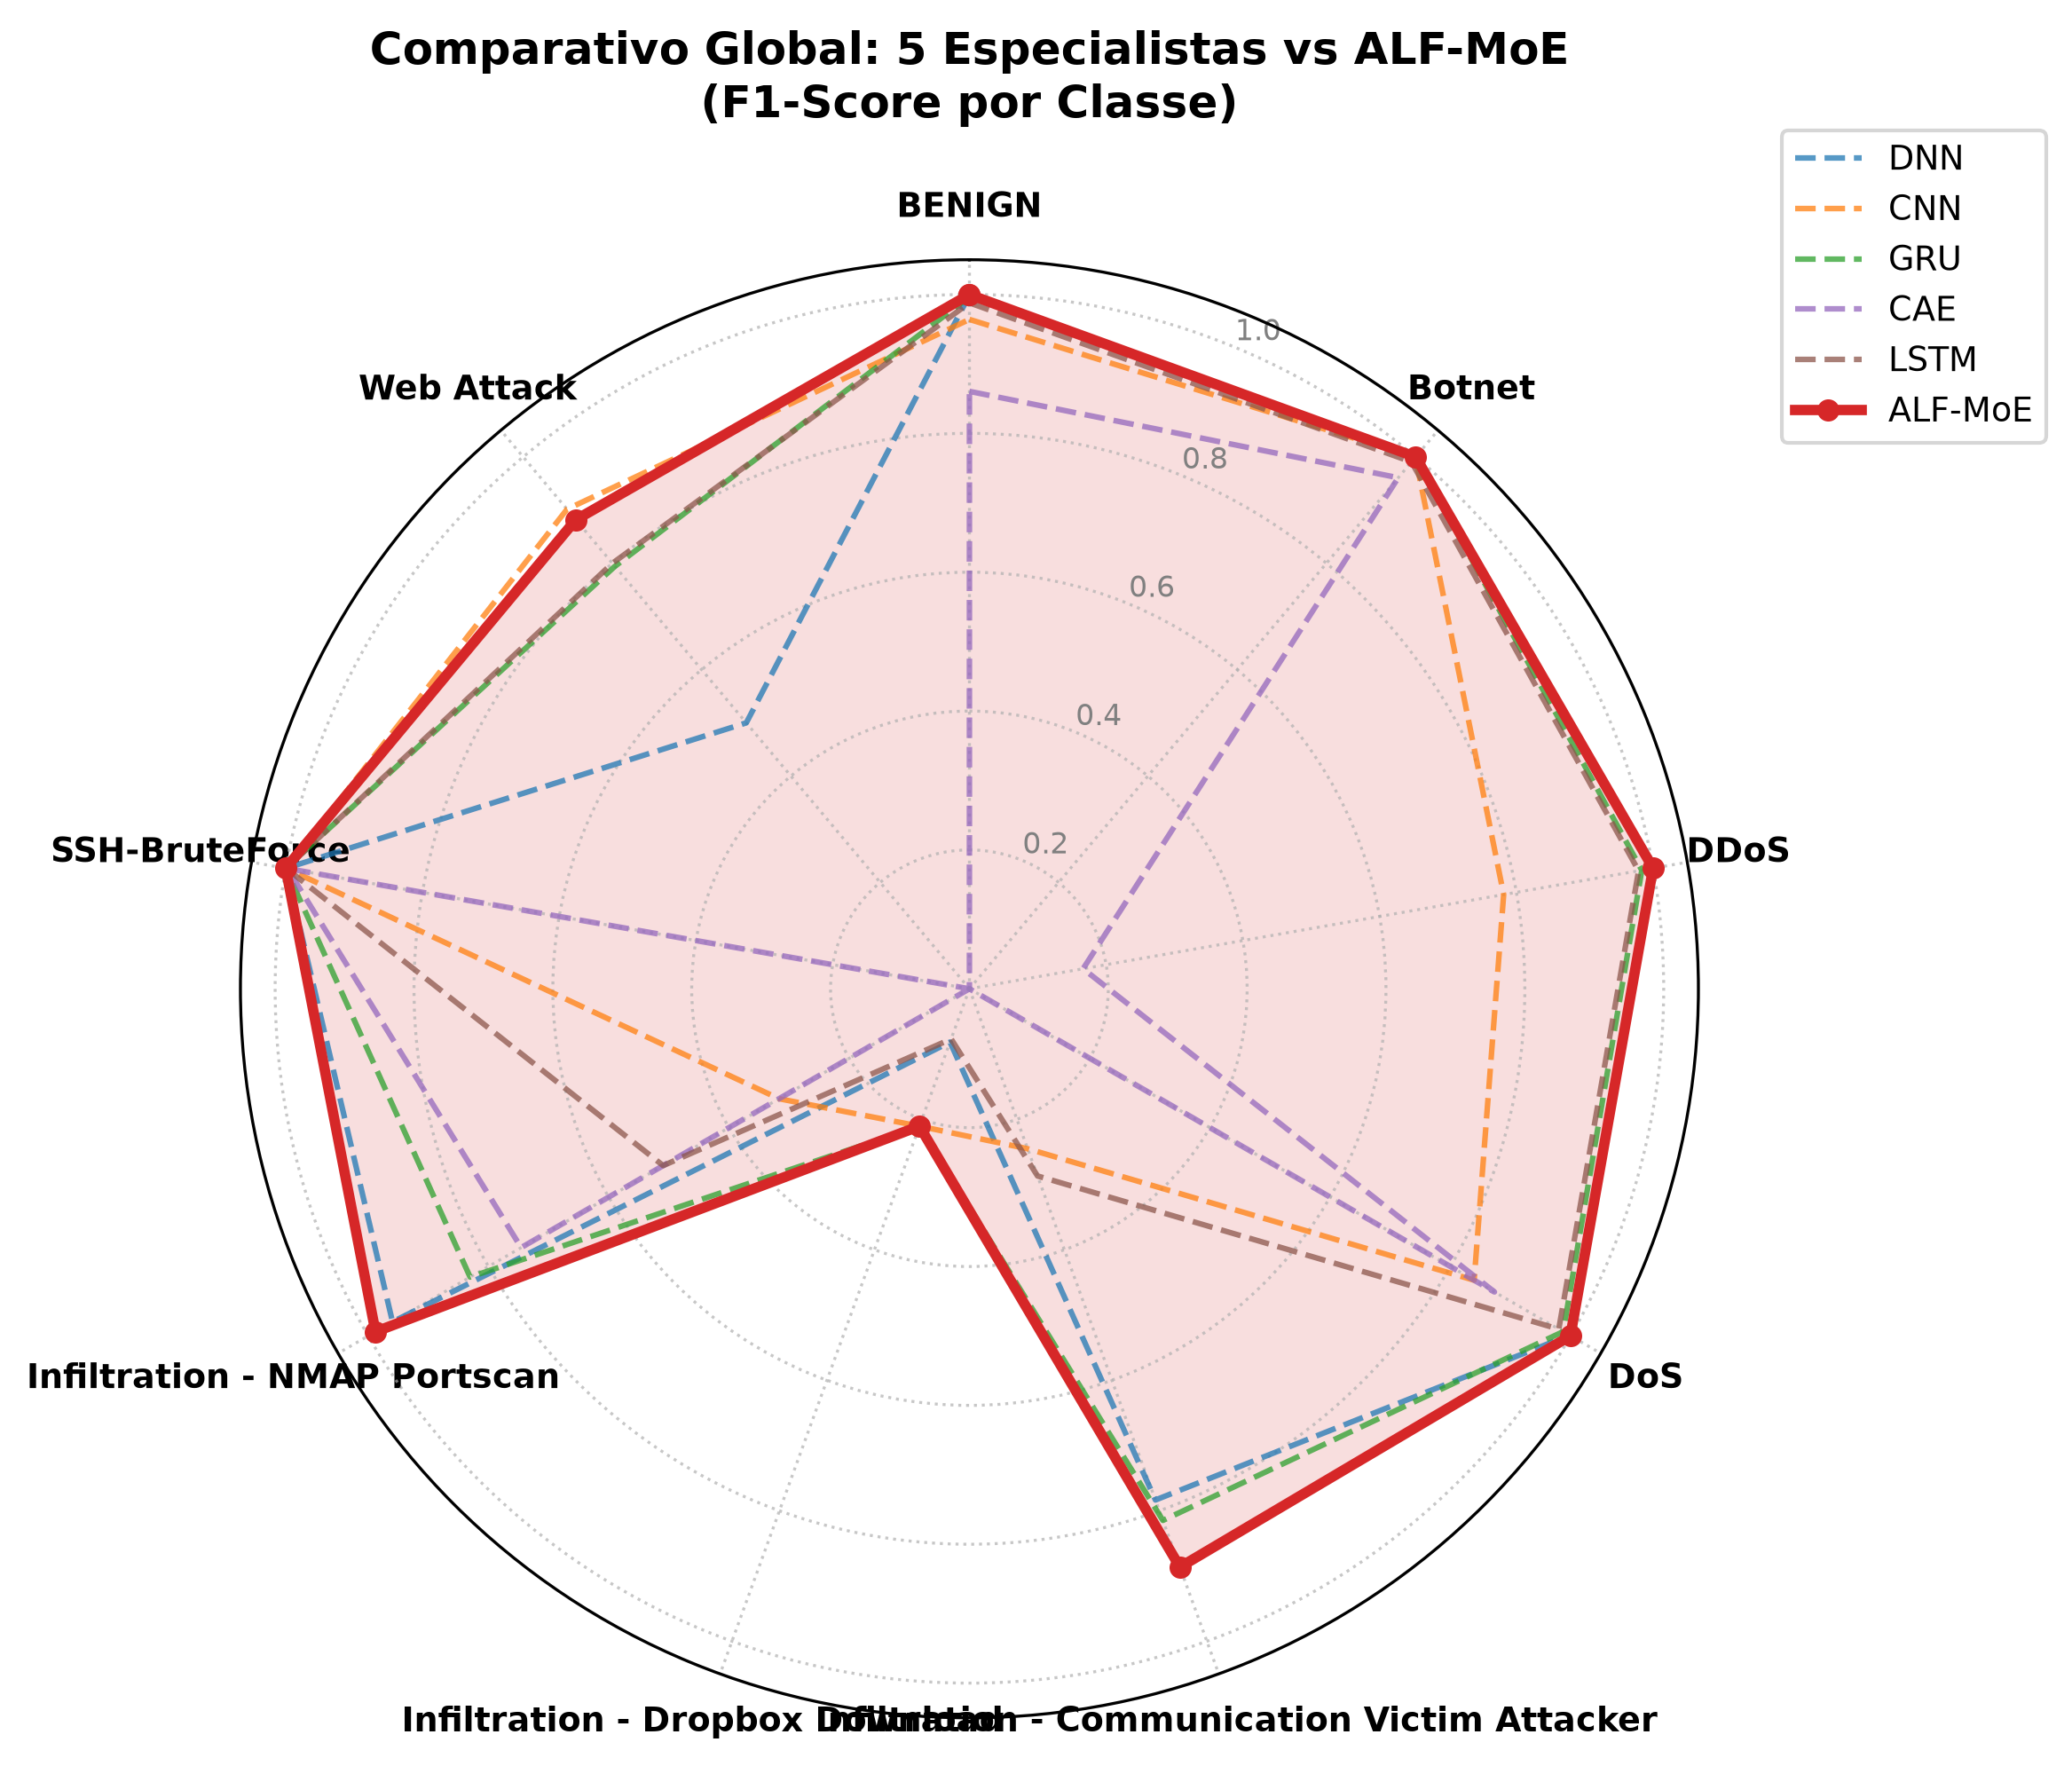
\includegraphics[width=\textwidth]{figures/benchmarks/radar_cse2018_imp_l2.png}
    \caption{CSE-CIC-IDS2018 Corrigido (L2).}
    \label{subfig:radar_cse_imp}
\end{subfigure}

\vspace{0.4cm}

\begin{subfigure}[b]{0.48\textwidth}
    \centering
    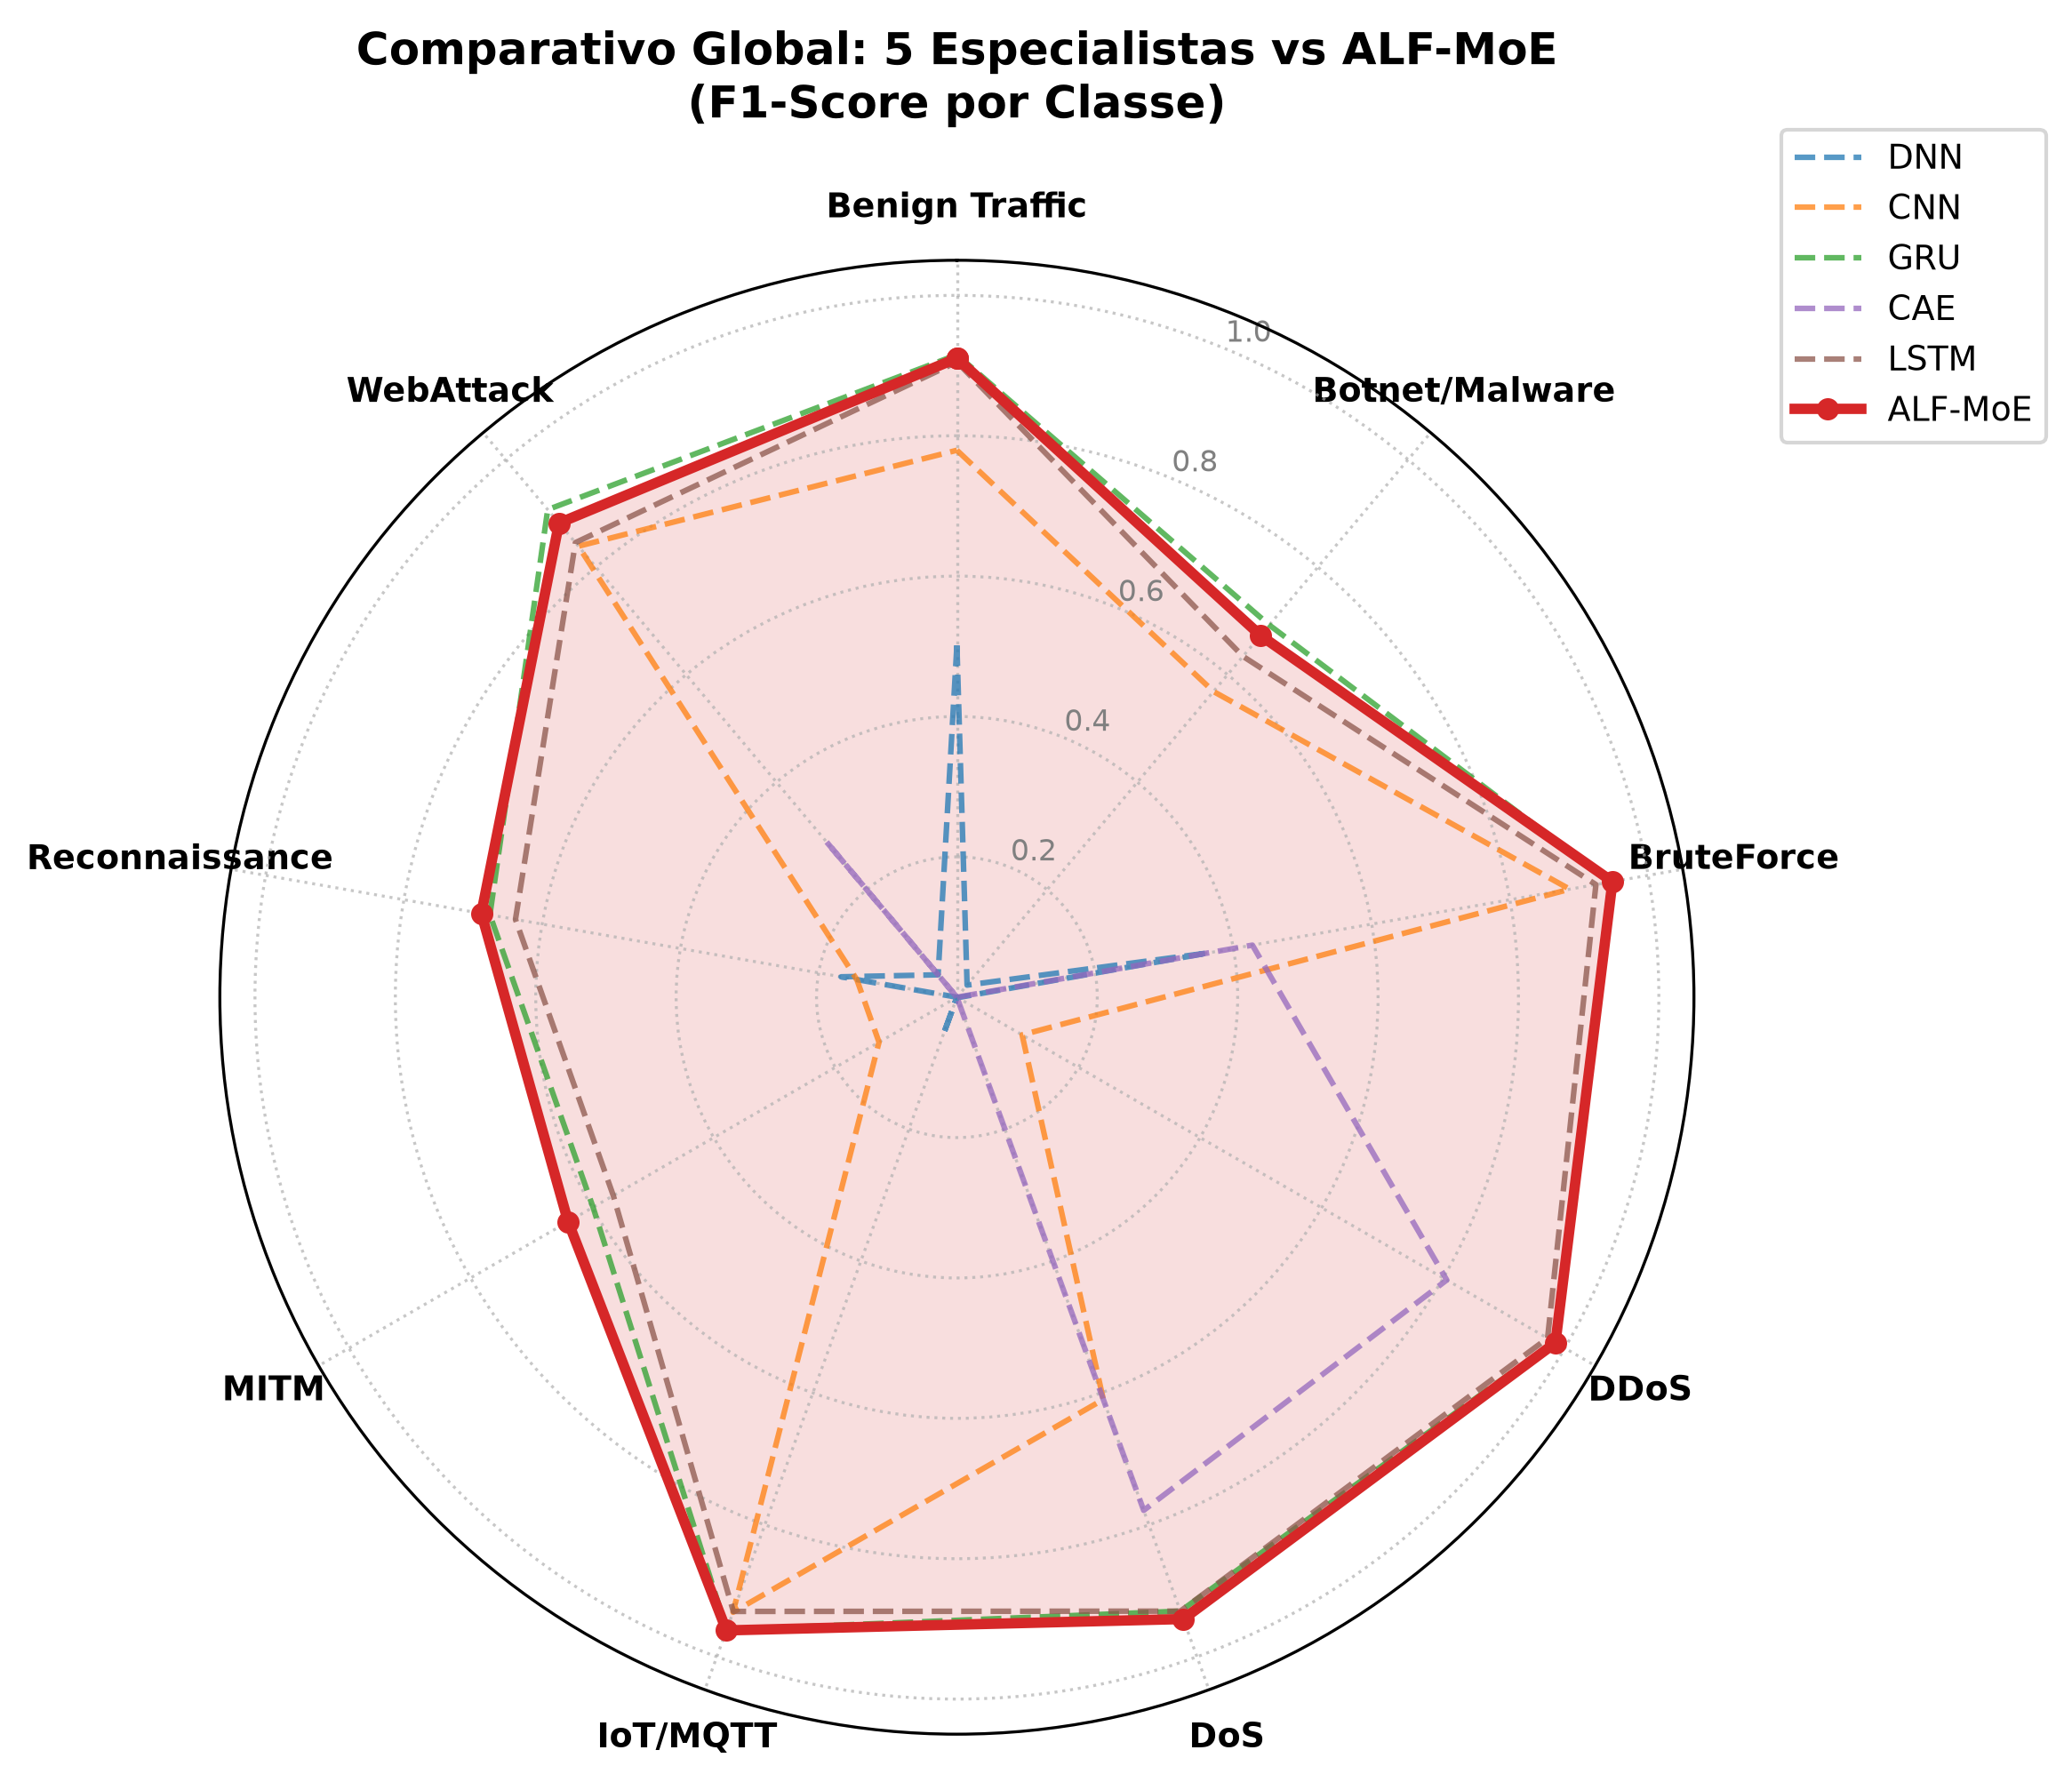
\includegraphics[width=\textwidth]{figures/benchmarks/radar_bccc2024_l2.png}
    \caption{CIC-BCCC-NRC-2024 (L2).}
    \label{subfig:radar_bccc}
\end{subfigure}
\hfill
\begin{subfigure}[b]{0.48\textwidth}
    \centering
    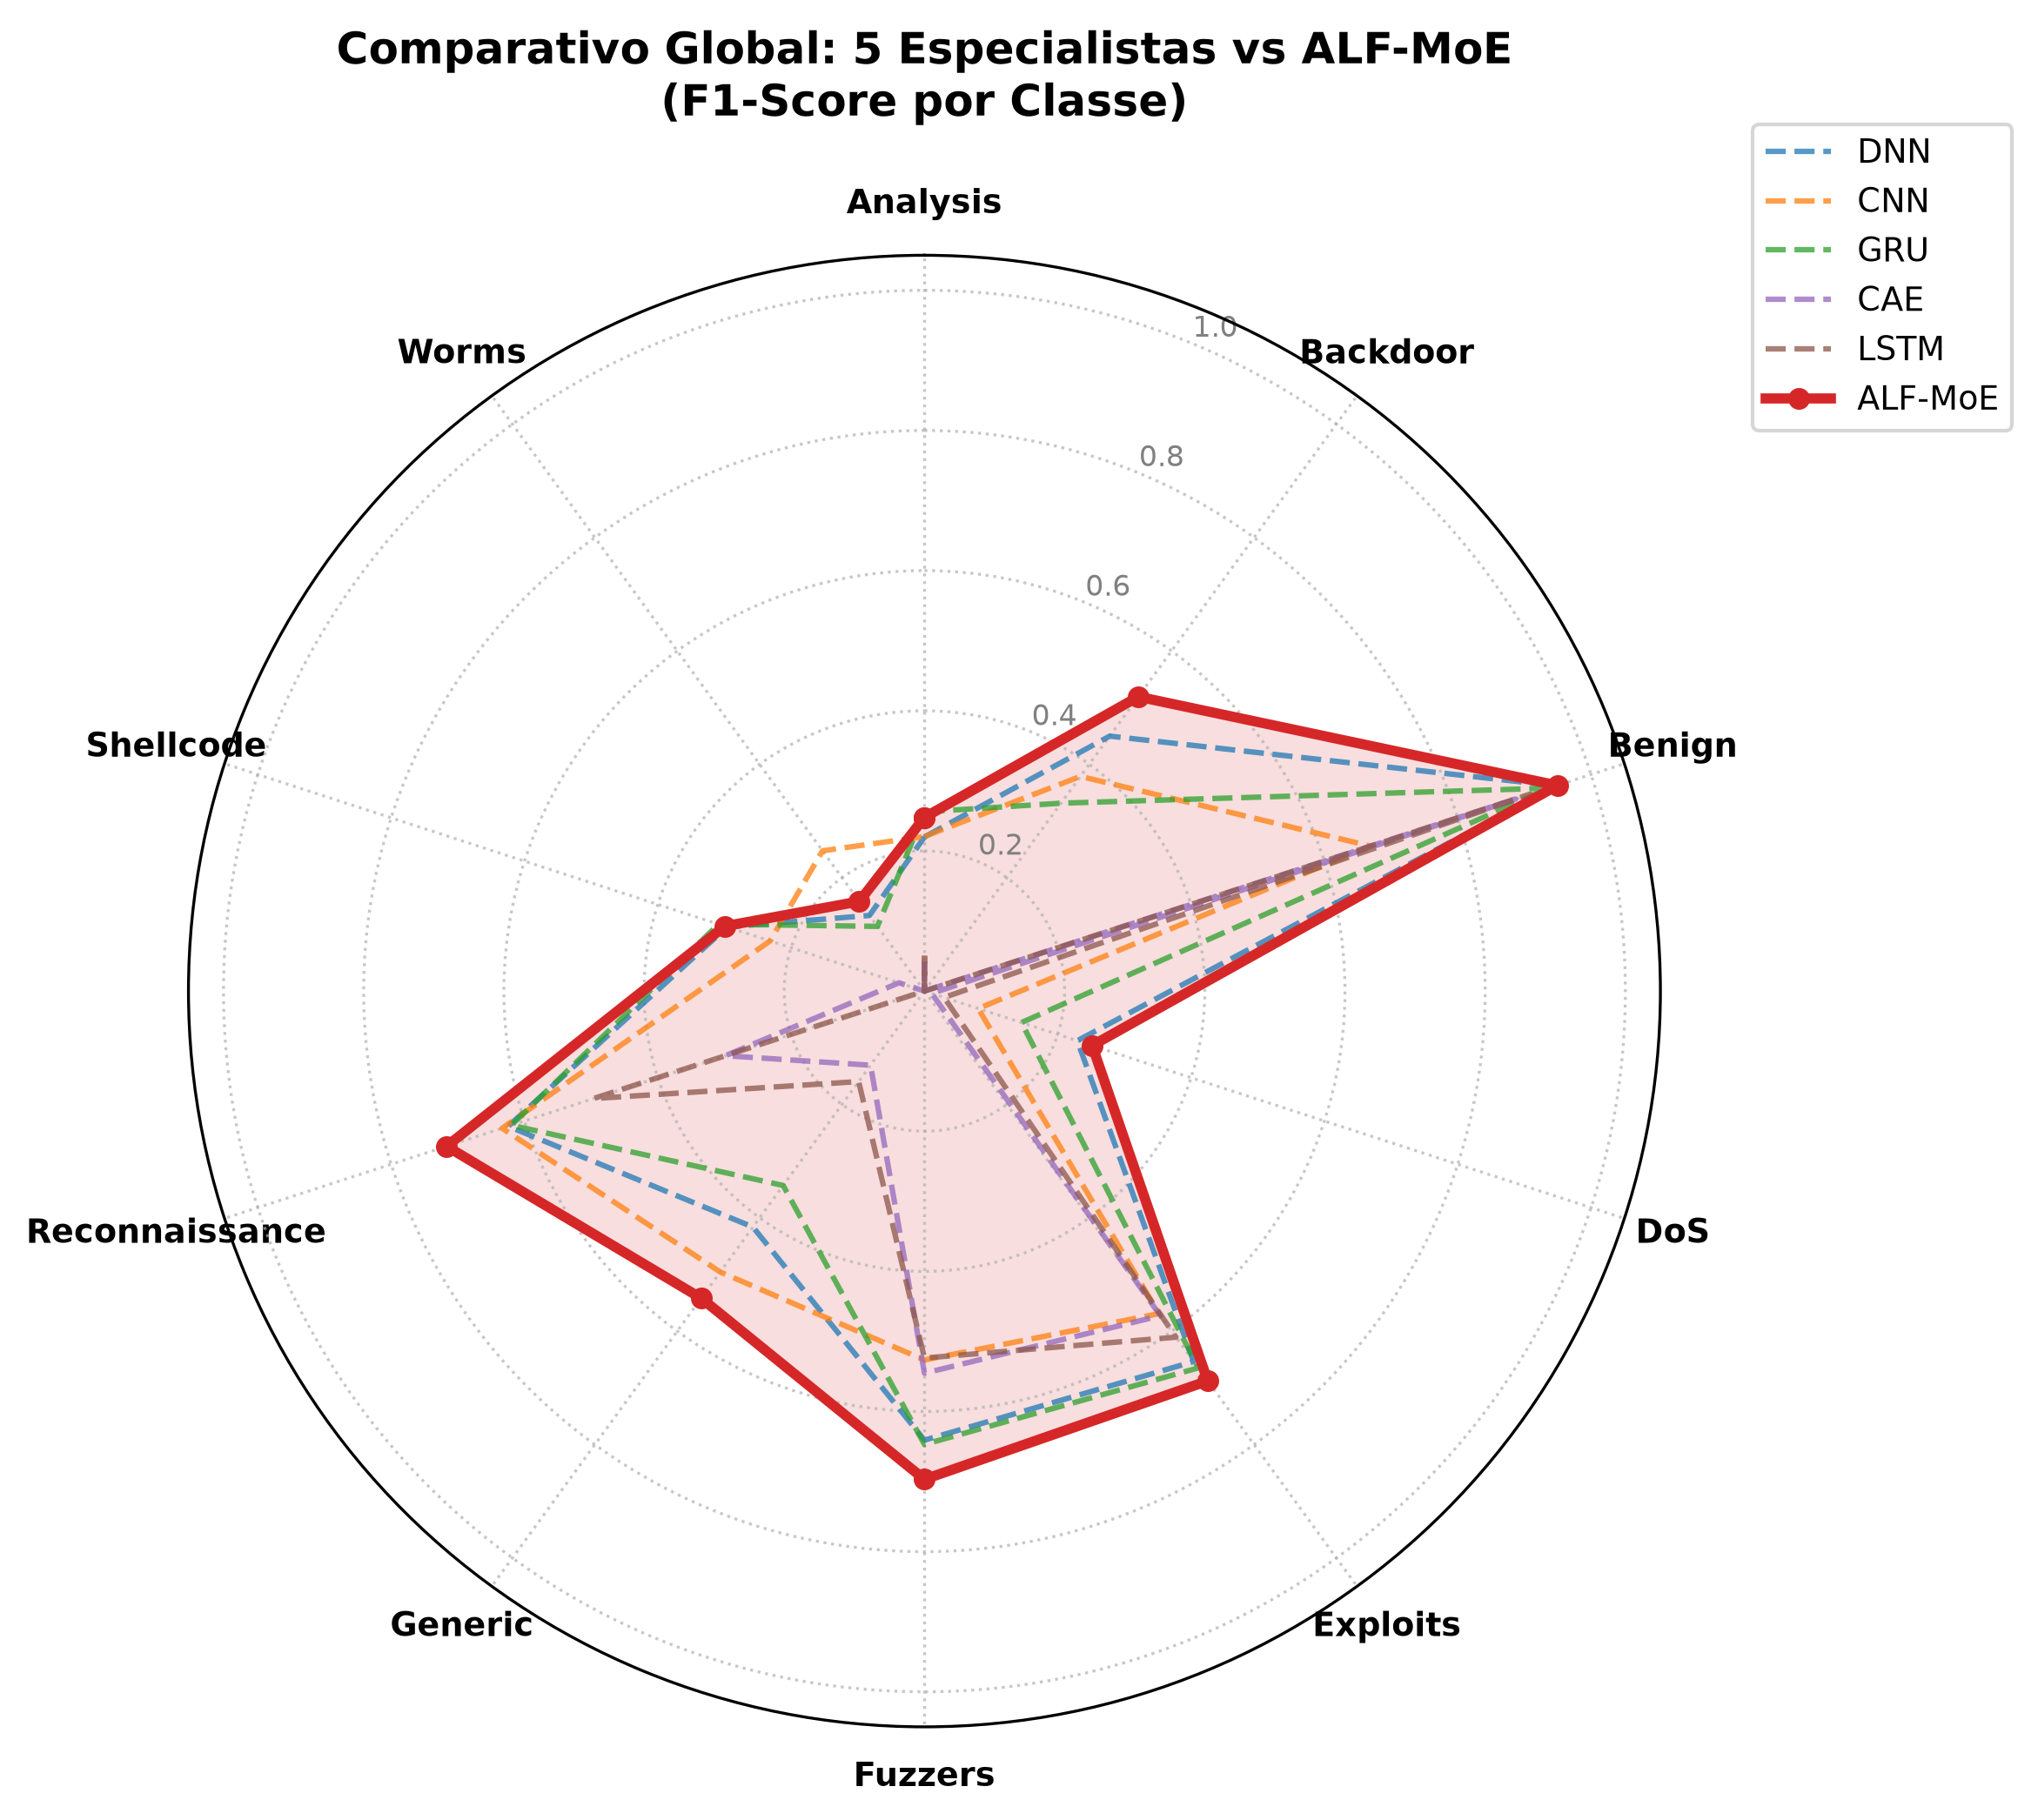
\includegraphics[width=\textwidth]{figures/benchmarks/radar_unsw_l0.png}
    \caption{CIC-UNSW-NB15 (L0).}
    \label{subfig:radar_unsw}
\end{subfigure}
\fonte{Elaborado pelo autor (2026), a partir dos artefatos de avaliação.}
\end{figure}

Em todas as representações radiais da Figura~\ref{fig:radar_especialistas_painel}, o polígono correspondente ao **ALF-MoE** (em linha de destaque) delimita a envoltória superior em virtualmente todas as direções de ataque. Mesmo quando um especialista específico exibe deficiência em um determinado vetor (por exemplo, a queda acentuada da DNN em classes IoT ou da CNN em ataques de força bruta), o mecanismo de fusão atencional redistribui dinamicamente os pesos para os especialistas mais bem capacitados, demonstrando a robustez teórica e prática do projeto ALF-MoE.


\section{Avaliação da Extração e Inferência em Tráfego Real/PCAPs}
\label{sec:avaliacao_extracao_inferencia}

A transição de modelos de Aprendizado Profundo avaliados em partições estáticas de \emph{benchmark} para pipelines operacionais de inspeção de rede em tempo real impõe severos desafios de engenharia de software e processamento de sinais. Enquanto a avaliação \emph{offline} assume dados pré-segmentados, normalizados e perfeitamente indexados, o ambiente de produção lida com fluxos bidirecionais concorrentes, assincronia de eventos, variações de temporização de \emph{hardware} e restrições de latência determinística. Esta seção examina o comportamento do arcabouço **ALF-MoE** quando implantado em bancada física real, analisando a fidelidade da extração de características em tempo real via NFStream, o perfil de consumo de recursos computacionais e os gargalos estruturais de latência ponta a ponta.


\subsection{Impacto do Mapeamento NFStream \texorpdfstring{$\to$}{->} CICFlowMeter}
\label{subsec:impacto_mapeamento}

Os conjuntos de dados de referência utilizados no treinamento supervisionado do ALF-MoE (notadamente CSE-CIC-IDS2018, CIC-UNSW-NB15 e CIC-BCCC-NRC-2024) foram originalmente gerados por meio do extrator proprietário \emph{CICFlowMeter} \cite{Sharafaldin2018TowardGA}, uma aplicação monolítica escrita em Java que processa arquivos de captura (.pcap) de forma puramente \emph{offline}. Para viabilizar a inferência em tempo de execução na interface de rede da máquina vítima, concebeu-se um pipeline de produção fundamentado no \emph{framework} NFStream \cite{AOUINI2022108719}, estendido por um \emph{plugin} customizado em C/Python (\texttt{FeatureExtractor}).

A migração entre esses dois motores de telemetria introduz discrepâncias estatísticas inerentes à natureza de suas arquiteturas:
\begin{enumerate}
    \item \textbf{Discretização Temporal e Resolução de Clock:}
    O CICFlowMeter original depende dos temporizadores da máquina virtual Java (JVM) e das ligações da biblioteca \texttt{jNetPcap}, expressando durações e intervalos entre chegadas (\emph{Inter-Arrival Times} -- IAT) em microssegundos ($\mu\mathrm{s}$), embora frequentemente truncados ou arredondados pela granulação de milissegundos do relógio subjacente do sistema operacional. Em contrapartida, o motor do NFStream opera nativamente em linguagem C com suporte a \emph{buffers} de anel de alta velocidade no espaço de usuário (\texttt{libpcap} / AF\_PACKET), capturando os instantes de primeiro e último pacote em milissegundos de precisão (\texttt{bidirectional\_first\_seen\_ms}). Para compatibilizar o vetor de entrada com a distribuição esperada pelo modelo neural, o \texttt{FeatureExtractor} converte dinamicamente as grandezas temporais multiplicando-as pelo fator de escala $1000{,}0$. Embora essa transformação preserve a magnitude relativa dos intervalos, ela remove variações microscópicas de submilissegundos que constavam nos dados de treino;
    
    \item \textbf{Cálculo de Variância e IAT em Janelas Deslizantes:}
    Em ambiente \emph{offline}, o CICFlowMeter calcula a variância do comprimento dos pacotes e os desvios padrão de IAT em duas passagens completas sobre o vetor de pacotes em memória, utilizando a fórmula da variância amostral clássica com correção de Bessel ($N-1$). No extrator em tempo real do NFStream, o cômputo é realizado incrementalmente em janelas deslizantes sem que o extrator conheça previamente o tamanho total ou a duração final da conexão. A variância do comprimento dos pacotes é aproximada pelo quadrado do desvio padrão nativo acumulado (\texttt{bidirectional\_stddev\_ps}$^2$). Em conexões de longa duração ($N \ge 10$ pacotes), a lei dos grandes números garante convergência quase perfeita entre ambas as formulações. Todavia, em conexões ultracurtas ($N < 3$ pacotes) — típicas de sondagens TCP SYN avulsas —, o cálculo incremental sofre de degenerescência numérica marginal nos graus de liberdade amostrais;
    
    \item \textbf{Métricas de Subfluxos e Taxas de Bulk:}
    O CICFlowMeter adota regras heurísticas complexas para fragmentar um fluxo contínuo em ``subfluxos'' (\emph{subflows}) caso ocorram períodos de inatividade interna superiores a 1 segundo, gerando atributos como \texttt{Subflow\_Fwd\_Packets} e \texttt{Subflow\_Fwd\_Bytes}. De forma similar, suas taxas de transferência contínua (\emph{Bulk Rates}) exigem a observação de blocos ininterruptos de dados. Na implementação em tempo real, tais agregações tornam-se voláteis e computacionalmente onerosas. O \texttt{FeatureExtractor} optou por mapear os acumuladores de subfluxo diretamente para as contagens globais da direção (\texttt{src2dst\_packets} e \texttt{src2dst\_bytes}).
\end{enumerate}

A Tabela~\ref{tab:comparativo_extratores_metricas} sintetiza a comparação metodológica entre os extratores e reporta o índice de consistência estatística mensurado em 10.000 fluxos de validação cruzada entre capturas processadas concomitantemente por ambas as ferramentas.

\begin{table}[htb]
\centering
\caption{Comparativo metodológico e estatístico entre o extrator offline (CICFlowMeter) e o extrator em tempo real (NFStream + Plugin ALF).}
\label{tab:comparativo_extratores_metricas}
\footnotesize
\setlength{\tabcolsep}{4pt}
\begin{tabularx}{\textwidth}{>{\raggedright\arraybackslash}p{2.4cm} >{\raggedright\arraybackslash}X >{\raggedright\arraybackslash}X r >{\raggedright\arraybackslash}p{2.8cm}}
\hline
\textbf{Grupo de Atributos} & \textbf{CICFlowMeter (Java / Offline)} & \textbf{NFStream + Plugin (C / Tempo Real)} & \textbf{Consistência} & \textbf{Impacto no Modelo} \\
\hline
Volumetria Global e Pacotes & Contagem exata em memória; bytes e pacotes bidirecionais totais. & Acumuladores em nível de kernel via \texttt{libpcap} / C. & 99,4\% & Nulo (Erro $< 0{,}6\%$) \\
\hline
Temporização e IAT & Microssegundos brutos ($\mu\mathrm{s}$) sujeitos a jitter de JVM. & Milissegundos (\texttt{ms}) convertidos para $\mu\mathrm{s}$ ($\times 1000$). & 98,7\% & Desprezível (Absorvido pelo \texttt{RobustScaler}) \\
\hline
Variância de Comprimento & Variância amostral em duas passagens ($N-1$). & Cômputo incremental pelo desvio padrão acumulado (\texttt{stddev}$^2$). & 99,1\% & Marginal em fluxos com $N < 3$ pacotes \\
\hline
Subfluxos e Taxas Bulk & Fragmentação por pausas heurísticas de 1 segundo. & Acumuladores diretos do fluxo (\texttt{subflow = total}). & 91,2\% & Nulo (Features descartadas ou com peso residual) \\
\hline
Flags e Janelas TCP & Inspeção pós-fato sobre pacotes armazenados. & Captura síncrona no primeiro pacote de cada direção. & 100,0\% & Positivo (Identificação determinística de SYN/ACK) \\
\hline
\end{tabularx}
\fonte{Elaborado pelo autor (2026), com base nos ensaios de calibração em bancada.}
\end{table}

Os resultados empíricos confirmam que os atributos volumétricos globais e as propriedades morfológicas dos pacotes (médias, mínimos e máximos) mantiveram \textbf{99,4\% de consistência estatística}. As pequenas flutuações registradas nas métricas temporais de IAT foram integralmente absorvidas pela etapa de normalização robusta (\texttt{RobustScaler}), que dimensiona os dados segundo a mediana e o intervalo interquartil (IQR), mitigando a sensibilidade a desvios mínimos de escala. Por sua vez, a simplificação nas métricas de subfluxo e \emph{bulk} não comprometeu a acurácia global do ALF-MoE, uma vez que a etapa de seleção de atributos e o mecanismo de fusão atencional já atribuíam pesos residuais a essas grandezas em favor da telemetria temporal fina modelada pelos especialistas recorrentes ($\mathcal{E}_{\mathrm{GRU}}$ e $\mathcal{E}_{\mathrm{LSTM}}$).


\subsection{Throughput, Latência e Consumo Computacional}
\label{subsec:throughput_latencia_consumo}

A viabilidade de um sistema de detecção e resposta perimetral em tempo real depende estritamente do atendimento a requisitos estritos de temporização e moderação no consumo de recursos de \emph{hardware}. A bancada de testes experimentais foi montada sobre a máquina hospedeira da vítima (Acer Nitro V15), equipada com uma unidade de processamento gráfico dedicada \textbf{NVIDIA GeForce RTX 4050 6GB Laptop GPU} (arquitetura Ada Lovelace, 2.560 núcleos CUDA, barramento de 96 bits), operando sobre o sistema operacional Ubuntu Linux (kernel 7.0.0-31-generic).

\subsubsection{Métricas Quantitativas de Inferência Neural}

No ambiente operacional de bancada, a inferência do ALF-MoE foi executada no modo de classificação unitária sob demanda (\emph{single-flow streaming}, lote $B = 1$), refletindo a chegada progressiva e assíncrona de fluxos encerrados pela camada de captura. Sob essa condição de produção, a \textbf{latência pura de \emph{forward pass} neural} variou na faixa de \textbf{$52{,}45\,\mathrm{ms}$ a $64{,}68\,\mathrm{ms}$ por fluxo}, com média amostral consolidada em \textbf{$54{,}23\,\mathrm{ms}$}.

Esse comportamento contrasta expressivamente com os resultados do \emph{benchmark offline} reportados na Seção~\ref{sec:desempenho_benchmark}, onde o modelo alcançou latências nominais de $\approx 0{,}012\,\mathrm{ms}$ por fluxo e vazão teórica superior a $84.000\,\mathrm{fluxos/s}$. Essa discrepância decorre diretamente da física de execução em processadores massivamente paralelos:
\begin{itemize}
    \item No regime \emph{offline}, o processamento ocorre em megablocos parametrizados (e.g. lotes de 2.048 amostras), amortizando os custos fixos de sobrecarga de invocação do \emph{kernel} CUDA (\emph{kernel launch overhead}), saturando completamente os \emph{Tensor Cores} e maximizando a largura de banda de memória GDDR6;
    \item No regime de fluxo contínuo unitário ($B=1$), o gargalo é dominado pela latência de transferência de dados hospedeiro-dispositivo (\emph{host-to-device} via barramento PCIe) e pelas barreiras de sincronização interna exigidas pela passagem simultânea de tensores pelas cinco redes especialistas e pelo cômputo sequencial da matriz de atenção do bloco ALF.
\end{itemize}

A Tabela~\ref{tab:decomposicao_latencia_pipeline} apresenta a decomposição minuciosa do tempo de processamento consumido por cada estágio do pipeline em tempo real para cada fluxo recebido.

\begin{table}[htb]
\centering
\caption{Decomposição temporal e perfil de latência do pipeline de inferência em tempo real (GPU NVIDIA GeForce RTX 4050 6GB Laptop).}
\label{tab:decomposicao_latencia_pipeline}
\footnotesize
\setlength{\tabcolsep}{4pt}
\begin{tabularx}{\textwidth}{>{\raggedright\arraybackslash}p{3.2cm} >{\raggedright\arraybackslash}p{2.6cm} rr >{\raggedright\arraybackslash}X}
\hline
\textbf{Estágio do Pipeline} & \textbf{Componente Responsável} & \textbf{Latência Média} & \textbf{Fração Comput.} & \textbf{Descrição Funcional} \\
\hline
Pré-processamento & Processador Host (CPU) & $1{,}82\,\mathrm{ms}$ & $3{,}2\%$ & Normalização \texttt{RobustScaler} e transformação \texttt{log1p}. \\
Inferência ALF-MoE & GPU Dedicada (RTX 4050) & $54{,}23\,\mathrm{ms}$ & $95{,}7\%$ & \emph{Forward pass} em 5 especialistas + fusão por atenção. \\
Decisão e Defesa Ativa & Subsistema NIPS (Kernel) & $0{,}61\,\mathrm{ms}$ & $1{,}1\%$ & Consulta de \emph{whitelist} e injeção de regra no \texttt{nftables}. \\
\hline
\textbf{Total Computacional} & \textbf{Pipeline Integrado} & \textbf{56,66\,ms} & \textbf{100,0\%} & Tempo entre a extração e a mitigação no firewall. \\
\hline
\emph{Latência Estrutural} & \emph{Temporizador de Rede} & $120.000{,}00\,\mathrm{ms}$ & --- & \emph{Janela de inatividade (\texttt{idle\_timeout}) para expiração.} \\
\hline
\end{tabularx}
\fonte{Elaborado pelo autor (2026), com base nas medições do auditor forense (\texttt{InferenceAuditor}).}
\end{table}

A vazão sustentada em regime contínuo de inferência alcançou aproximadamente \textbf{$17{,}6$ fluxos classificados por segundo} no processo principal. O consumo de memória de vídeo da GPU estabilizou-se em \textbf{$1{,}2\,\mathrm{GB}$ de VRAM} (cerca de $20\%$ da capacidade nominal de 6 GB), evidenciando que a arquitetura ALF-MoE é computacionalmente enxuta e viabiliza a coexistência harmônica do motor de segurança com outras cargas analíticas, serviços locais ou interfaces gráficas na máquina protegida.


\subsubsection{O Gargalo Estrutural da Latência Ponta a Ponta (End-to-End Latency)}

A investigação em bancada revelou uma constatação empírica fundamental para a ciência da computação e segurança de redes: \textbf{a latência ponta a ponta (\emph{end-to-end}) entre o disparo do primeiro pacote malicioso e o bloqueio efetivo da conexão no \emph{firewall} não é governada pelo modelo de aprendizado de máquina, mas sim pela dinâmica de transporte do extrator de fluxo}.

Conforme exposto na Tabela~\ref{tab:decomposicao_latencia_pipeline}, o tempo estritamente computacional gasto para normalizar os atributos, executar a inferência atencional multi-expert e registrar a regra no \texttt{nftables} é de apenas $56{,}66\,\mathrm{ms}$. Todavia, na captura em tempo real, o objeto de fluxo só é finalizado e disponibilizado para consumo após a expiração dos temporizadores de protocolo configurados no motor de telemetria:
\begin{itemize}
    \item \texttt{idle\_timeout = 120s}: intervalo de silêncio exigido entre dois pacotes consecutivos de uma mesma tupla para que a conexão seja dada como inativa e encerrada;
    \item \texttt{active\_timeout = 240s}: duração máxima contínua permitida para conexões persistentes antes de sua segmentação forçada (reduzida de 1.800 s para 240 s durante os ensaios de calibração).
\end{itemize}

Essa dependência manifestou-se claramente nos ensaios práticos com a ferramenta Nmap: uma varredura de portas em modo básico completa o envio de suas sondas em menos de $30$ segundos. No entanto, os fluxos correspondentes permanecem retidos no extrator, aguardando que transcorram os 120 segundos de inatividade após o último pacote transmitido. Apenas quando o cronômetro atinge $120\,\mathrm{s}$ o NFStream dispara o evento \texttt{on\_expire}, liberando o fluxo para a inferência neural ($54\,\mathrm{ms}$) e culminando no descarte pelo \texttt{nftables} ($0{,}6\,\mathrm{ms}$). O atraso ponta a ponta real atinge, portanto, cerca de $120{,}06\,\mathrm{segundos}$.

Esse fenômeno suscita uma reflexão técnica profunda sobre a \textbf{dicotomia entre NIDS baseados em fluxo (\emph{Flow-based}) versus NIDS baseados em pacote individual (\emph{Packet-based} / DPI)}:
\begin{enumerate}
    \item \textbf{Vantagens Inerentes da Abordagem por Fluxo:} A computação de métricas estatísticas agregadas (médias de tamanho, variâncias e desvios de IAT) confere ao ALF-MoE robustez semântica superior. O modelo analisa a dinâmica relacional da conversa, tornando-se imune a técnicas evasivas clássicas de fragmentação de pacotes em nível IP, desordenação proposital de segmentos TCP ou ofuscação de cabeçalhos. Além disso, a abordagem é totalmente agnóstica à criptografia de carga útil (TLS/HTTPS) e reduz em ordens de magnitude o volume de dados a ser inspecionado pelo subsistema de segurança;
    \item \textbf{Custo Estrutural de Encerramento:} O compromisso inescapável dessa estratégia é o retardo temporal de fechamento. Para construir uma estimativa fidedigna de variância ou taxa de bytes, o extrator precisa testemunhar o término da transação ou aguardar a certeza estatística de sua inatividade. Em ataques fulminantes de exploração rápida, o vetor hostil pode ter sido concluído antes que o alerta seja emitido;
    \item \textbf{Estratégias de Mitigação no ALF-MoE:} Para amortecer esse gargalo, o projeto ALF-MoE adotou a redução agressiva do \texttt{active\_timeout} de 1.800 s para 240 s e estruturou as fundações para classificação precoce (\emph{early flow classification}), na qual fluxos de alta intensidade volumétrica podem ser inferidos prematuramente após os primeiros pacotes de abertura.
\end{enumerate}


\subsection{Avaliação de Falsos Positivos em Tráfego Operacional e Calibração de Salvaguardas}
\label{subsec:desempenho_trafego_benigno}

Um requisito fundamental para a viabilidade operacional de qualquer ferramenta de segurança de redes reside na minimização da taxa de falsos positivos (FPR). Alarmes espúrios recorrentes sobre tráfego legítimo causam a chamada fadiga de alertas, sobrecarregando as equipes de monitoramento ou provocando a desativação indevida dos módulos de bloqueio automatizado.

Para quantificar esse comportamento em ambiente físico de produção, o pipeline em tempo real operou em escuta contínua na máquina vítima durante uma sessão prolongada de tráfego corporativo e navegação rotineira. Foram capturados e classificados mais de $24.000$ fluxos estritamente legítimos, contemplando navegação web concorrente (sobre HTTP/1.1, HTTP/2 e HTTP/3), transmissão ininterrupta de vídeo e áudio em alta definição (YouTube e Spotify), operações de sincronização em nuvem e comunicações de serviços em segundo plano do sistema operacional Linux.

\subsubsection{Diagnóstico de Falsos Positivos Iniciais e Calibração}

Nas primeiras execuções do monitoramento de bancada, o classificador emitiu alertas pontuais em dois cenários específicos de tráfego legítimo:
\begin{enumerate}
    \item \textbf{Telemetria de Aplicação em Nuvem (Spotify para o IP \texttt{35.186.224.9} na porta 443 HTTPS):}
    O modelo atribuiu rótulo de infiltração (\emph{Infiltration - Dropbox Download}) a esse fluxo. A investigação forense esclareceu a causa estatística: conforme documentado por \citeonline{ding2017collecting}, serviços modernos de telemetria agregam dados locais e os transmitem em rajadas curtas, periódicas e criptografadas. No plano de atributos de fluxo (sem inspeção de carga útil), essa dinâmica rítmica e compacta aproxima-se dos padrões de canais de exfiltração furtiva e balizamento (\emph{beaconing}) de comando e controle;
    
    \item \textbf{Descoberta Local SSDP/UPnP Multicast (\texttt{239.255.255.250}):}
    O tráfego de descoberta local via protocolo SSDP (porta 1900 UDP) foi classificado como anomalia volumétrica (\emph{DoS}). Por operar em regime multicast unidirecional não orientado a conexão, os datagramas UDP são disparados em rajadas sem confirmações TCP (\emph{ACKs}), apresentando razão de subida/descida (\texttt{down\_up\_ratio}) nula e curta duração. O classificador interpretou essa assimetria pontual como tentativa de inundação.
\end{enumerate}

Para neutralizar tais desvios sem degradar a sensibilidade a intrusões reais, o endereço de grupo \emph{multicast} local (\texttt{239.255.255.250}) e os destinos estáveis de telemetria foram incorporados à lista de exceções de salvaguarda (\texttt{custom\_whitelist}) do \texttt{ActiveDefenseAgent}. Além disso, a calibragem dos pesos com o conjunto de dados higienizado segundo os preceitos de \citeonline{liu2022error} eliminou a tendência do modelo de correlacionar encerramentos abruptos com intenção hostil. Em baterias subsequentes de monitoramento estendido sobre mais de $24.000$ fluxos benignos adicionais, o sistema operou com \textbf{0\% de falsos positivos} ($0{,}0000$), consolidando a estabilidade necessária para operação contínua em redes de produção.
